% Copyright (C) 2014-2017 by Thomas Auzinger <thomas@auzinger.name>

\documentclass[draft,final]{vutinfth} % Remove option 'final' to obtain debug information.

% Load packages to allow in- and output of non-ASCII characters.
\usepackage{lmodern}        % Use an extension of the original Computer Modern font to minimize the use of bitmapped letters.
\usepackage[T1]{fontenc}    % Determines font encoding of the output. Font packages have to be included before this line.
\usepackage[utf8]{inputenc} % Determines encoding of the input. All input files have to use UTF8 encoding.

% Extended LaTeX functionality is enables by including packages with \usepackage{...}.
\usepackage{amsmath}    % Extended typesetting of mathematical expression.
\usepackage{amssymb}    % Provides a multitude of mathematical symbols.
\usepackage{mathtools}  % Further extensions of mathematical typesetting.
\usepackage{microtype}  % Small-scale typographic enhancements.
\usepackage[inline]{enumitem} % User control over the layout of lists (itemize, enumerate, description).
\usepackage{multirow}   % Allows table elements to span several rows.
\usepackage{booktabs}   % Improves the typesettings of tables.
\usepackage{subcaption} % Allows the use of subfigures and enables their referencing.
\usepackage[ruled,linesnumbered,algochapter]{algorithm2e} % Enables the writing of pseudo code.
\usepackage[usenames,dvipsnames,table]{xcolor} % Allows the definition and use of colors. This package has to be included before tikz.
\usepackage{nag}       % Issues warnings when best practices in writing LaTeX documents are violated.
\usepackage{todonotes} % Provides tooltip-like todo notes.
\usepackage{hyperref}  % Enables cross linking in the electronic document version. This package has to be included second to last.
\usepackage[acronym,toc]{glossaries} % Enables the generation of glossaries and lists fo acronyms. This package has to be included last.

\usepackage{listings}
\lstset{
	language=bash,
	basicstyle=\footnotesize, 
	breakatwhitespace=false
}

% Define convenience functions to use the author name and the thesis title in the PDF document properties.
\newcommand{\authorname}{Bernhard Gößwein} % The author name without titles.
\newcommand{\thesistitle}{Designing a Framework gaining Repeatability for the OpenEO platform} % The title of the thesis. The English version should be used, if it exists.

% Set PDF document properties
\hypersetup{
    pdfpagelayout   = TwoPageRight,           % How the document is shown in PDF viewers (optional).
    linkbordercolor = {Melon},                % The color of the borders of boxes around crosslinks (optional).
    pdfauthor       = {\authorname},          % The author's name in the document properties (optional).
    pdftitle        = {\thesistitle},         % The document's title in the document properties (optional).
    pdfsubject      = {Subject},              % The document's subject in the document properties (optional).
    pdfkeywords     = {a, list, of, keywords} % The document's keywords in the document properties (optional).
}

\setpnumwidth{2.5em}        % Avoid overfull hboxes in the table of contents (see memoir manual).
\setsecnumdepth{subsection} % Enumerate subsections.

\nonzeroparskip             % Create space between paragraphs (optional).
\setlength{\parindent}{0pt} % Remove paragraph identation (optional).

\makeindex      % Use an optional index.
\makeglossaries % Use an optional glossary.
%\glstocfalse   % Remove the glossaries from the table of contents.

% Set persons with 4 arguments:
%  {title before name}{name}{title after name}{gender}
%  where both titles are optional (i.e. can be given as empty brackets {}).
\setauthor{}{\authorname}{}{male}
\setadvisor{Ao.Univ.Prof. Dipl.-Ing. Dr.techn.}{Andreas Rauber}{}{male}

% For bachelor and master theses:
%\setfirstassistant{Ao.Univ.Prof. Dipl.-Ing. Dr.techn.}{Andreas Rauber}{}{male}
\setfirstassistant{Dr.}{Tomasz Miksa}{}{male}
%\setthirdassistant{Pretitle}{Forename Surname}{Posttitle}{male}

% For dissertations:
%\setfirstreviewer{Pretitle}{Forename Surname}{Posttitle}{male}
%\setsecondreviewer{Pretitle}{Forename Surname}{Posttitle}{male}

% For dissertations at the PhD School and optionally for dissertations:
%\setsecondadvisor{Pretitle}{Forename Surname}{Posttitle}{male} % Comment to remove.

% Required data.
\setaddress{Vorderer Ödhof 1, 3062 Kirchstetten}
\setregnumber{01026884}
\setdate{21}{12}{2018} % Set date with 3 arguments: {day}{month}{year}.
\settitle{\thesistitle}{Entwurf eines Frameworks zur Unterstützung von Reproduzierbarkeit für die OpenEO Plattform} % Sets English and German version of the title (both can be English or German). If your title contains commas, enclose it with additional curvy brackets (i.e., {{your title}}) or define it as a macro as done with \thesistitle.
\setsubtitle{}{} % Sets English and German version of the subtitle (both can be English or German).

% Select the thesis type: bachelor / master / doctor / phd-school.
% Bachelor:
%\setthesis{bachelor}
%
% Master:
\setthesis{master}
\setmasterdegree{dipl.} % dipl. / rer.nat. / rer.soc.oec. / master
%
% Doctor:
%\setthesis{doctor}
%\setdoctordegree{rer.soc.oec.}% rer.nat. / techn. / rer.soc.oec.
%
% Doctor at the PhD School
%\setthesis{phd-school} % Deactivate non-English title pages (see below)

% For bachelor and master:
\setcurriculum{Software Engineering and Internet Computing}{Software Engineering and Internet Computing} % Sets the English and German name of the curriculum.

% For dissertations at the PhD School:
%\setfirstreviewerdata{Affiliation, Country}
%\setsecondreviewerdata{Affiliation, Country}

\newcolumntype{L}[1]{>{\centering\arraybackslash}l{#1}}

\begin{document}

\frontmatter % Switches to roman numbering.
% The structure of the thesis has to conform to
%  http://www.informatik.tuwien.ac.at/dekanat

\addtitlepage{naustrian} % German title page (not for dissertations at the PhD School).
\addtitlepage{english} % English title page.
\addstatementpage

%\begin{danksagung*}


%\end{danksagung*}

\begin{acknowledgements*}
To my girlfriend Viola: Thank you very much for helping me through the stressful days of working on the thesis and for providing breaks and diversions when I needed them.\\ \\
To my family: Thank you for supporting me through my whole studying time and for motivating me to go on with the thesis. \\ \\
To my colleagues of the Remote sensing research group: Thank you for patiently waiting for me to finish my studies and letting me work on a thesis within the OpenEO project. \\ \\
To my colleagues at EODC: Thank you for providing me all resources I requested and letting me implement the solution on your system. \\ \\
Last but not least to my supervisors Andreas Rauber and Tomas Miksa for always quickly replying on questions and providing me with constructive feedback. 
\end{acknowledgements*}

\begin{kurzfassung}
Publikationen in den Bereichen der Geodäsie und Geoinformation sind oft, aus diversen Gründen, nicht reproduzierbar. Daher fand in den letzten Jahren ein Umdenken in Bezug auf reproduzierbare Publikationen in den computergestützten Geowissenschaften statt. Die Problematik für Wissenschaftler dieser Forschungsbereiche ist die große Anzahl an unterschiedlichen Anbietern, fehlende Datenversionierung und intransparente Anbieter Services. Existierende Literatur beschränkt sich auf konkrete Anbieter und Forschungsbereiche. Dabei wird der Fokus mehr auf die Ausführung des selben Auftrages als auf Reproduzierbarkeit gelegt. Um diese zu ermöglichen ist es notwendig die Daten und die Bearbeitung dieser zu identifizieren. Dabei fehlt es der Geodäsie und Geoinformation an einem allgemeinen Konzept dies sowohl für Wissenschaftler als auch für Anbieter zu ermöglichen. Das Ziel dieser Arbeit ist es eine allgemeine Lösung zur Reproduzierbarkeit in den Geowissenschaften zu erstellen, indem die Daten und deren Bearbeitung automatisch identifizierbar gemacht werden. Dafür wird eine vollständige Lösung innerhalb des Horizon 2020 Projektes OpenEO konzipiert, welche im Earth Observation Data Centre for Water Resources Monitoring (EODC) Anbieter implementiert wird. Die Research Data Allience (RDA) Empfehlungen bezüglich Datenzitierbarkeit werden in diesem Kontext angewendet. Um die Bearbeitung der Daten einzufangen wird das VFramework Konzept angewandt. Die Implementierung in EODC wird über vordefinierter Szenarien für Geowissenschaftler evaluiert.    
\end{kurzfassung}


\begin{abstract}
Studies show that many areas of earth observation sciences lack in creating reproducible research. In the last years there was an extensive movement towards policies defining reproducibility for geoscientists. The diverse set of data providers, the lack of data versions and processing systems without transparency of environment meta-data are responsible for scientists not being able to reproduce experiments. Existing solutions focus on re-execution and are specific for certain work-flows and back ends. To reproduce an experiment, the input data and the work-flow have to be identifiable. The earth observation community has no general solution that can be easily applied by the providers and is simple to use for scientists. The aim of this thesis is a general concept of reproducibility in the context of the earth observation community, by applying automatic data identification and work-flow capturing methods. Therefore, a complete system is implemented within the Horizon 2020 OpenEO project, which is a unified abstraction layer standard for earth observation data providers. In doing so, the Earth Observation Data Centre for Water Resources Monitoring (EODC) back end is extended applying the Resarch Data Allience (RDA) data identification recommendations. To capture the processing work-flow the VFramework is implemented into the solution. The prototype is evaluated by predefined scenarios of scientists using EODC to examine the viability of the prototype.    
\end{abstract}

% Select the language of the thesis, e.g., english or naustrian.
\selectlanguage{english}

% Add a table of contents (toc).
\tableofcontents % Starred version, i.e., \tableofcontents*, removes the self-entry.

% Switch to arabic numbering and start the enumeration of chapters in the table of content.
\mainmatter

\chapter{Introduction}\label{Introduction}
\section{Motivation}\label{Motivation}
Over the last decades remote sensing agencies have increased the variations of data processing and therefore the amount of resulting data. The complexity of the experiments leads researchers to use external services for the workflow. These circumstances makes it hard for scientists to provide the necessary information to enable reproducibility. Scientists just create a description of the work-flow and the used satellite identifier to describe experiments. To preserve the data for further usage in the future it is necessary to have citable data and processes on the data to ensure long-term reproducibility \cite{6352411}. Reproducibility is discussed in many scientific areas such as computer science, biology and in computational geoscience. In \cite{reprovsrepli} "reproducing" an experiment is defined by running a second different experiment, which results in the same conclusion as the first experiment. The more the second experiment differs from the first, the more information is gained by it. It is needed to provide additional evidence about the outcome of an experiment. Replicability is the re-run of the same methods of the first experiment with the aim of checking if the described methods lead to the claimed results\cite{reprovsrepli}. According to \cite{Ostermann2017AdvancingSW} where the reproducibility and replicability of scientific papers in geoscience got tested, only half of the publications were replicable and none of them reproducible. In \cite{Thestateofreproducibility} a survey of geoscientific readers and authors of papers got executed, with the goal of finding reasons for the lack of reproducibility in earth observation sciences. One of the results is that even though 49\% of the participants responded that their publications are reproducible, only 12\% of them have linked the used code. The understanding of open reproducible research is different among the participating scientists in a way that the interpretation is more related to repeatability and replicability. The main reasons for the lack of reproducibility in computational geoscience are:

\begin{enumerate}
	\item Insufficiently described methods 
	\item No persistent data identifier
	\item Legal concerns
	\item The impression that it is not necessary
	\item Too Time consuming
\end{enumerate} 

Reproducing geoscientific papers failed by the different individual interpretation of the described approach in the publication. If the code is published with the publication, alternative software versions produced unequal results e.g. a different versions of the CRAN library in R resulted in a different result. The vast majority of issues on reproducing results are required changes of code and a deeper understanding of the procedures e.g. if functions are deprecated and the code has to be modified for using new functions. In some cases issues occur, which are system dependent and related to the usage of random access memory and installation libraries of the operating system \cite{Thestateofreproducibility}. In \cite{Thestateofreproducibility} resulting images of the research are reproduced and compared with the result of the original execution. Figure \ref{fig:motivation} shows an example of a result confrontation of the original experiment and the replicated experiment. The map shows spatially gridded biomass burning and was originally published  in \cite{bg-13-3225-2016}. Even though the resulting numbers of the reproduction remains the same as the original one, the different aspect ratio changes the appearance of the resulting image and therefore might lead to a different interpretation.

\begin{figure}[h]
	\centering
	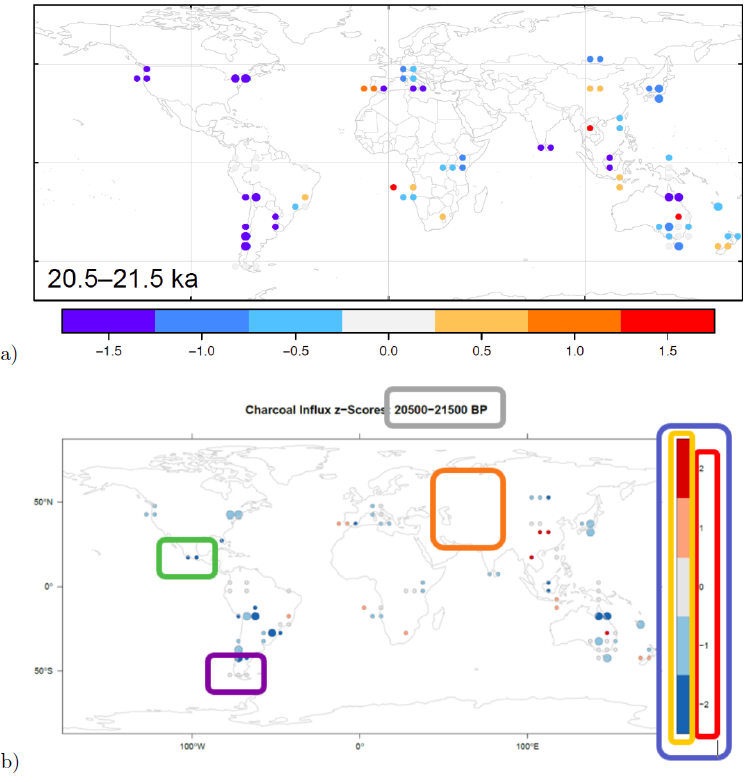
\includegraphics[scale=0.5]{motivation_example}
	\caption{Example of a comparison of the original result (a) and the replicated result (b). The boxes are highlighting the differences of the map. The blue box shows the misplacement of the legend, the purple box shows different colour of results, the red box shows a different data type of the legend numbers, the grey box shows a different labeling, the orange box highlights differences in the background map, the yellow box shows a different number of classes and the green box shows results that were not in the original figure \cite{Thestateofreproducibility}.}
	\label{fig:motivation} % \label has to be placed AFTER \caption (or \subcaption) to produce correct cross-references.
\end{figure} 

\section{Problem Description}\label{Problem}
The vast majority of data used in earth observation sciences are retrieved and provided via Service Oriented Architecture (SOA) interfaces. Data providers like Google Earth Engine (GEE\footnote{https://earthengine.google.com}) and Earth Observation Data Centre for Water Resources Monitoring (EODC\footnote{https://www.eodc.eu}) host a Web Application Programming Interface (API) for data download and processing data. These services are used to define the experiment work-flow, the definition of the used data, the execution and the retrieval of the results. Therefore, researcher are not in full control of the code execution and the environment of their experiments, since the information about the work-flow environment of the experiment is not accessible for the scientists. Used external dependencies for processing the earth observation data can not be accessed. The services act as black boxes to the researchers with no possibility to get versions of the used packages to calculate the resulting images. The situation leads to the problem, that researchers are not capable of describing the experiments in a way that they can be reproduced. \\
Input data of a typical remote sensing work-flow is defined by satellite data of a specified satellite type filtered by a temporal and a spatial extent. The raw satellite data is preprocessed by the back end provider, so that there is a global dataset. Geoscientists using the same satellite identifier can have different results after executing the same experiment, if the provider updated the way the data is preprocessed. An examle for this is the format update of ESA in 2017 of the Sentinel 1 dataset, which affected old data records, see \footnote{https://sentinel.esa.int/web/sentinel/missions/sentinel-1/news/-/article/sentinel-1-update-of-product-format}. When scientists use the dataset of a data provider, there is no possibility to see changes in the preprocessing algorithm. Therefore, data versions are not visible for the researcher. This leads to the problem that scientists are not capable of identifying the used input data, which is a necessity for reproducibility. 
\todo{Talk about big data of Geoscience and how big it is...}
\todo{maybe find better example of data update than format problems...}
%Due to a different range of functionality and a difference between the endpoints of the providers, it is great afford to create a workflow for more than one provider. The OpenEO project has the goal to be an abstraction layer above different EO data providers. Further information on the software architecture of the project is defined in the project proposal (\cite{openeo}) and in Section \ref{Related Work}. During the creation time of this thesis there is no consideration of repeatability in the OpenEO architecture. Verification of work-flows for users of OpenEO is not in the agenda of the OpenEO project. Generalized layers have the opportunity to be implemented in a way that makes processes and data scientifically verifiable and reproducible, as it handles data and processes on the data in a standardized way for different providers. Even though the range of functionality and the API endpoints are well-defined in the OpenEO core-API, the contributing content providers (OpenEO back ends) will have different underlying software execution environments. The used technology of an OpenEO back end will evolve in the future, hence it can lead to different results on the same workflow execution. Considering the following: A scientist runs an experiment using OpenEO as research tool and gets an arbitrary result. The same scientist runs the same experiment with the same input data some months later and gets a slightly different result. The question occurs, why are the results distinct? Has the used data changed, has the user accidentally submitted different code or has some underlying software inside the back end provider changed. Adding a possibility for the users of OpenEO to gain this information is an important feature for the scientific community. The aim of this thesis is to design an extension to OpenEO, so that users are able to retrieve provenance data about a job re-execution \cite{openeo}. 

\section{Aim of the Work}\label{Aim}\label{Use Cases}

The following sections define use cases to validate the design proposed in this thesis. They describe scenarios focused on scientific work-flows that are currently not achievable, but shall be accomplish-able with the solution of this thesis. This thesis uses the term "job" for the definition of a work-flow, since it is common in earth observation science.

\subsection{Example Experiment}\label{example}

This section describes an example of an experiment that a remote sensing scientist wants to execute. The example will be used throughout the thesis for better illustration of the concepts. It is used in the Use Cases in the following sections. \\
The input data of the experiment is Sentinel 2 data developed by the European Space Agency (ESA). The area of interest is the province south tyrol. More specifically the bounding area in the "EPSG:4326" projection with the coordinates for an north-west corner of (10.288696, 46.905246) and an south-east corner of (12.189331, 45.935871). The time of interest is the month May of the year 2017. In this example the scientist is working on vegetation dynamics and wants to know what the state of the vegetation of south tyrol was in the beginning of 2017. Therefore the minimum of the Normalized Difference Vegetation Index (NDVI\footnote{https://earthobservatory.nasa.gov/features/MeasuringVegetation/measuring\_vegetation\_2.php}) is calculated on the data selection. It is derived from the difference between near-infrared (which reflects vegetation strongly) and red light (which vegetation absorbs). So for every pixel of the satellite image the NDVI value is calculated for every day of May 2017. Then the 31 images for May 2017 are reduced to one by taking the minimum NDVI value of each pixel. Figure \ref{fig:example} shows the result of the running example execution.\\

The execution of the experiment consists of the following steps:

\begin{enumerate}
	\item Selecting the Sentinel 2 data records
	\item Filtering the Sentinel 2 records by the extent of south tyrol. \\(10.288696, 46.905246) - (12.189331, 45.935871) on "EPSG:4326" projection.
	\item Filtering the Sentinel 2 records by May 2017.
	\item Calculate NDVI for all days of May 2017.
	\item Reduce by the minimum value of May 2017.
	\item Interpret the resulting image.
\end{enumerate}

\begin{figure}[h]
	\centering
	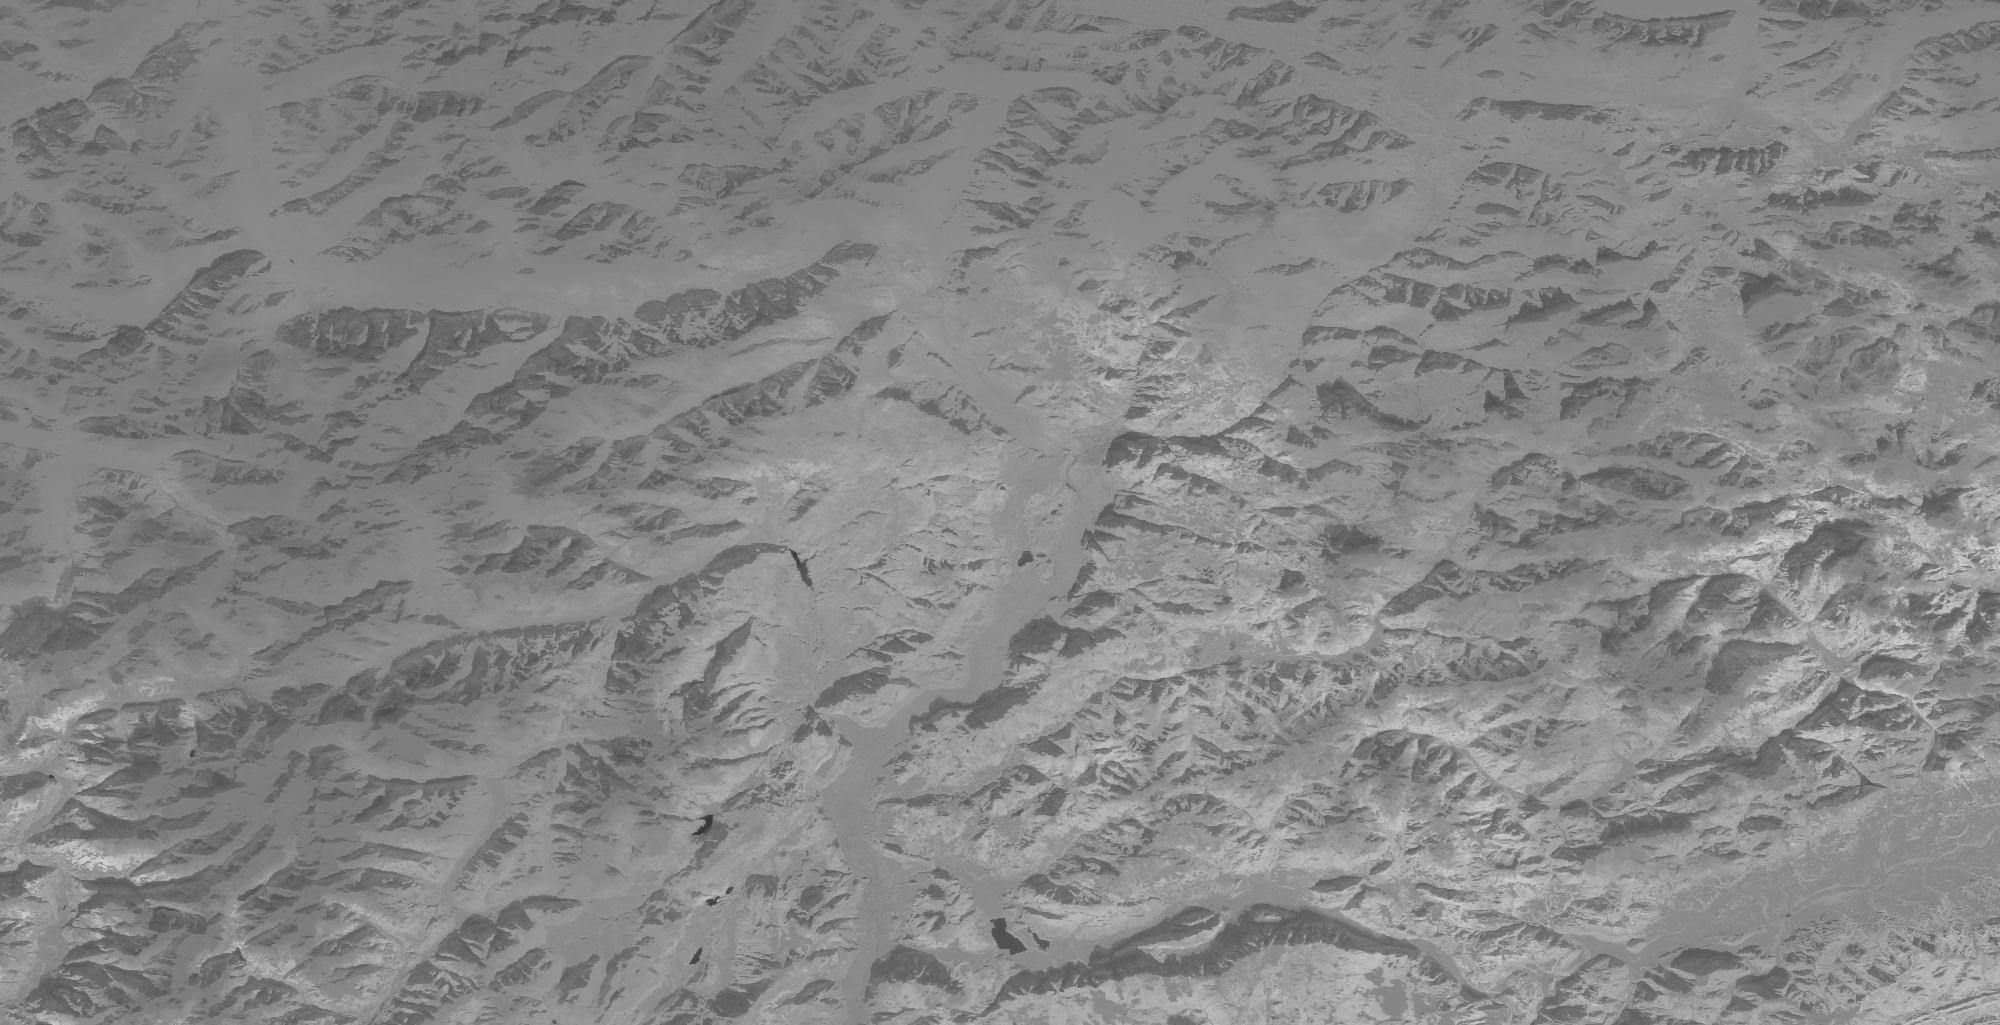
\includegraphics[width=\textwidth]{openeo_example_output}
	\caption{Resulting image of the running example.}
	\label{fig:example} % \label has to be placed AFTER \caption (or \subcaption) to produce correct cross-references.
\end{figure}


\subsection{Re-use of input data}\label{UseCase1}
\begin{figure}[h]
	\centering
	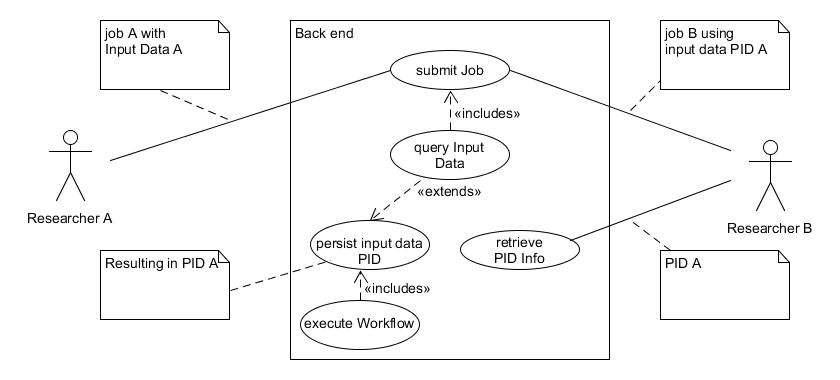
\includegraphics[width=\textwidth]{usecase1}
	\caption{Overview of the first Use Case.}
	\label{fig:usecase1} % \label has to be placed AFTER \caption (or \subcaption) to produce correct cross-references.
\end{figure}
The first use case is about the re-use of input data between job executions. Reproducible methods are especially important for the scientific community. Since scientists are likely to build on results and methods of publications, this is a scenario to make the re-use simpler. In this case a scientist wants to create a publication by running the example, described in Section \ref{example} on an earth observation back end. The back end generates a persistent data identifier (PID) for the input data of the experiment. After that the scientist publishes the results and cites the input data with the resulting PID. The PID redirects to a human readable landing page that provides meta information about the dataset. Another scientist also interested in the vegetation of south tyrol wants to use the same input data but chooses a different approach of processing it (e.g. maximum instead of minimum). Hence, the input data PID can be used to re-use the same data. The back end has to be capable of resolving the PID automatically to let the user work with the same input data for a new work-flow. The data provider need to persist the data defined by a PID even if the preprocessing of the data changes in the future.    

\begin{itemize}
	\item \textbf{Input Data A}: Sentinel 2 data of the area of south tyrol in May 2017. 
	\item \textbf{Job A}: Taking the \textbf{minimum} NDVI of the area of south tyrol in May 2017. 
	\item \textbf{Job B}: Taking the \textbf{maximum} NDVI of the area of south tyrol in May 2017.
\end{itemize}

An overview of the use case can be viewed in Figure \ref{fig:usecase1}. \\

The scenario sequence of actions is summarized in the following steps: \\

\begin{enumerate}
	\item Researcher A runs job A at the back end.
	\item Researcher A retrieves the used input data PID of job A.
	\item Researcher A cites the input data with the PID in a publication.
	\item Researcher B uses the same input data, by applying the data PID of job A for job B.  
\end{enumerate}

\subsection{Providing job execution Information}\label{UseCase2}
\begin{figure}[h]
	\centering
	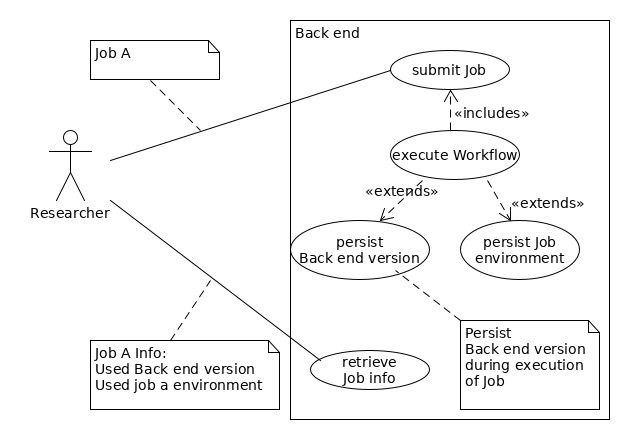
\includegraphics[width=\textwidth]{usecase2}
	\caption{Overview of the second Use Case}
	\label{fig:usecase2} % \label has to be placed AFTER \caption (or \subcaption) to produce correct cross-references.
\end{figure}

This use case is like the first one, but is exclusively about job dependent environment information. The scientist can automatically get environment data about the job execution e.g. used software packages and their versions. Motivation for this is to add transparency of the job processing for the users, so that researchers can describe their processes in more detail. It can help geoscientists to understand why results differ from executions in the past. An overview of the use case can be viewed in Figure \ref{fig:usecase2}. 
The scenario sequence of actions is summarized in the following steps: \\
\begin{enumerate}
	\item Researcher runs an experiment (job A) at a back end.
	\item Researcher wants to describe the experiment environment.
%	\item Back End Developer releases a new version.   
%	\item Back End Developer runs test jobs to find differences.
\end{enumerate}

\subsection{Compare different job executions}\label{UseCase3}
\begin{figure}[h]
	\centering
	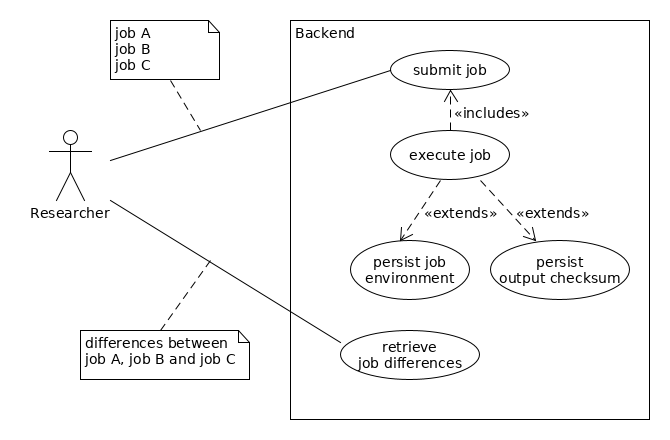
\includegraphics[width=\textwidth]{usecase3}
	\caption{Overview of the third Use Case}
	\label{fig:usecase3} % \label has to be placed AFTER \caption (or \subcaption) to produce correct cross-references.
\end{figure}
The third use case is dedicated to the comparison of job executions. The goal is to add a possibility for geoscientists to compare different jobs not only by their results, but on the way they were executed. The comparison is applied between a job execution and another job execution on the same back end. Therefore, the processing implementation and the input data has to be identifiable. To make the comparison interesting to the users additional meta-data is added to the job environment data e.g. an output checksum. For usability reasons the comparison needs to be easy to apply and easy to understand, therefore accessible in the context of the user. In addition to the previous conditions a visualization of the differences for the users can lower the access barrier for them to use the feature. An overview of this use case can be viewed in Figure \ref{fig:usecase3}.
The scenario sequence of actions is summarized in the following steps: \\

\begin{itemize}
	\item \textbf{Job A}: Taking the minimum NDVI of the area of south tyrol in May 2017. 
	\item \textbf{Job B}: Taking the minimum NDVI of the area of south tyrol in May 2017.
	\item \textbf{Job C}: Taking the maximum NDVI of the area of south tyrol in May 2017.
\end{itemize}

\begin{enumerate}
	\item Researcher runs an experiment (job A) at a back end.
	\item Researcher re-runs the same experiment (job B).
	\item Researcher runs a different experiment (job C).   
	\item Researcher receives a comparison of the jobs (A, B, C) by their environment and outcome.
\end{enumerate}

\subsection{Research Questions}\label{research question}

The expected outcome of this thesis is to discover and develop a framework for making repeatability conceivable in the earth observation community. This enables users to re-execute work-flows and validate the result, so that differences on the processing or the data are accessible for the users. To achieve this goal a model for capturing the environment of the back ends has to be discovered and implemented. Since the solution is implemented within the open source Earth Observation (OpenEO) project (details see Section \ref{OpenEO}), it shall conclude in recommendations for the OpenEO project on how to improve re-execution validation for the users and how it can be achieved. Considering the problem description and the scenarios above, the following research questions can be formulated:

\begin{itemize}
	\item \textbf{How can an earth observation job re-execution be applied like the initial execution?}
	\begin{itemize}
		\item How can the used data be identified after the initial execution?
		\item How can the used software of the initial execution be reproduced?
		\item What data has to be captured when?
		\item How can the result of a re-execution in future software versions be verified?
	\end{itemize}
	\item \textbf{How can the equality of a earth observation job re-execution results be validated?}
	\begin{itemize}
		\item What are the validation requirements?
		\item How can the data be compared?
		\item How can changes of the earth observation back end environment be recognized?
		\item How can differences in the environment between the executions be discovered?
	\end{itemize}
\end{itemize}



\section{Methodological Approach}\label{Method}
The use cases defined in the previous section require specific changes to the components of an earth observation back end. The following list describes the parts of the suggested solution briefly: 


\begin{enumerate}
	\item \textbf{Data Identification}
	In order to accomplish the capturing of processing workflows described in the use cases in Section \ref{Use Cases}, the input data has to be identifiable. In order to achieve this the recommendations of the RDA (see \cite{rauber2016identification}) have to be implemented by adding versioning and query databases. 
	
	\item \textbf{Process Versioning}
	To accomplish the verification of different process executions, the process has to be identifiable. Therefore, a versioning of the process code can be used to persist different states of the code. The thesis is for an OpenSource project and the code of the back ends are published at Github, so Git is used as the tool to capture the code state. 
		
	\item \textbf{User Endpoints}
	The interface for users has to be implemented so that the use cases can be executed. Therefore, client applications have to be modified. The used programming language in this thesis is Python\footnote{https://www.python.org}.
\end{enumerate}

\section{Structure of Work}\label{Structure}
The following sections are structured as followed:\\
Chapter 2 gives an overview of related scientific activities in the area of reproducibility in the earth observation sciences and reproducibility in other areas with similar objectives. \\
%Chapter 3  describes the technologies and concepts that are used in the implementation of this thesis. This chapter provides an overview of the EODC back end used for the implementation.\\
Chapter 3 provides the concept to address the research questions defined in Section \ref{Aim}.  This is the theoretical definition of what has to be implemented in the OpenEO project.\\
Chapter 4 has a detailed explanation to the proof of concept prototype implementation and how the concept of chapter 3 was realized for the EODC back end. \\
Chapter 5 dives into the evaluation of the implementation by applying the use cases to the implementation of chapter 4.\\
Chapter 6 summarizes the outcome of the implementation and evaluation. It contains a discussion on results achieved, open issues and future work. \\

\chapter{Related Work}\label{Related Work}

This chapter describes the related work of the thesis. In the following the reader gets informed about basic concepts related to the prototype implementation. The information is structured in subsections, where each represents different technologies or concepts. \\The first section presents the concepts behind reproducibility in computer science. \\
The second section describes the state of reproducibility in earth observation science. \\
The third section presents concepts related to data identification. \\ 
The fourth section consists of existing tools that can be used to achieve reproducibility. \\
The last section of this chapter describes the OpenEO project further and more specifically the EODC back end, which is used for the proof of concept implementation in Chapter \ref{Implementation}.    


\section{Reproducibility}\label{Reproducibility}
According to \cite{6064509}, reproducibility is defined as a new experiment based on an original experiment by an independent researcher in the manner of the original experiment. The aim of reproducibility is to gain additional evidence on the result of the original result, by creating an independent experiment that shows similar results. Repetition is the re-run of the exact same experiment with the same method, same environment and very similar result. The aim of the repetition is to check if the methods described in a publication are resulting in the purposed outcome. 
Achieving reproducibility is a common problem in all scientific areas. It is an issue of the whole scientific community to produce results that are reproducible. Therefore in \cite{10.1371/journal.pcbi.1003285} there are ten rules defined to gain a common sense about reproducibility in all science areas. They consist of the basic idea that every result of interest has to be associated with a process and data used. External programs have to be persisted as well as custom script versions. The usage of version control is recommended. In addition there is a rule defined to make the scripts and their results publicly available \cite{10.1371/journal.pcbi.1003285}. 
Reproducibility is the key element of The Fourth Paradigm published in \cite{noauthororeditorfourth}. It leads to the term eScience, which has the aim of bringing science and computer technologies closer together. The general concept is to enable scientific procedures in the new information technologies used by data intensive sciences. The expected result of eScience is to get all scientific papers publicly available including the necessary data and work-flows so that scientists are able to have a fast interaction with each other \cite{noauthororeditorfourth}. 
eScience has the potential to enable a boost in scientific discovery by providing approaches to make digital data and work-flows citable. The publication \cite{Rauber2015RepeatabilityAR} discusses a common way of reaching the goal formulated above. It describes an approach to look at whole research processes by introducing Process Management Plans, other than limiting it to data citation. The capturing, verification and validation of the input data for a computational process is demonstrated within the paper \cite{Rauber2015RepeatabilityAR}.
Computer sciences have the issue of a high amount of published papers that do not provide enough information to make them reproducible. The problem will not be solved by the scientists that need to do additional effort to make reproducibility doable, but by providing new tools for scientists that allow it automatically as stated in \cite{MIKSA201725}. There are some additional issues on reproducibility in computer science e.g. in the case that used software technologies are deprecated and not available any more. Therefore, persisting the execution context is critical to achieve a re-execution of the experiment. One proposed concept of doing so is the VFramework described in more detail in the method Section \ref{Related Work}. 
The PRIMAD model defines a set of variables that define an experiment. The relationship of the original execution to a re-execution can be visualized by noticing changes of the variables in the re-execution. The following variables of an experiment are used to describe the relationship to the second experiment according to \cite{primad}:

\begin{itemize}
	\item \textbf{P} Platform / Execution Environment / Context (e.g. Python 2.7, Windows 10,\dots) \\
	\item \textbf{R} Research Objectives / Goals (e.g. sorting the input) \\
	\item \textbf{I} Implementation / Code / Source-Code (e.g. script in Python) \\
	\item \textbf{M} Methods / Algorithms (e.g. quick sort) \\
	\item \textbf{A} Actors / Persons (e.g. researcher that is executing the experiment) \\
	\item \textbf{D} Data (input data and parameter values)   (e.g. input data that is to be sorted) 
\end{itemize}
If there is another experiment that is different on every variable to the original one, but has the same method (M) and goal (R), then it is a reproducing experiment \cite{primad}. 
\\  
Data citation is a key issue of reproducing results of past experiments. Preserving the exact process without persisting the original data is no positive effect for the scientific community. If the data used in an experiment is not available anymore, or not specified explicit enough then there is no chance of reproducing it no matter how much information about the execution was persisted. In earth observation persisting the data for reproducibility in the future is an issue discussed in \cite{6352411}.Gaining data identification in digital sciences has an official working group named Working Group on Data Citation (WGDC), which created 14 recommendations on data citation further explained in Section \ref{Data Identification}.

 \subsection{PROV-O}\label{PROV}
In 2003 the World Wide Web Consortium published the PROV model as a standard for provenance definitions. It is defined by twelve different documents. In the context of this thesis the PROV Ontology (PROV-O) is the most relevant \cite{733f89c65e4844f9aabcae1c276a5602}. 
PROV-O is a standard language using OWL2 Web Ontology. It is designed as a lightweight concept to be used in a broad spectrum of applications. 

\begin{figure}[h]
	\centering
	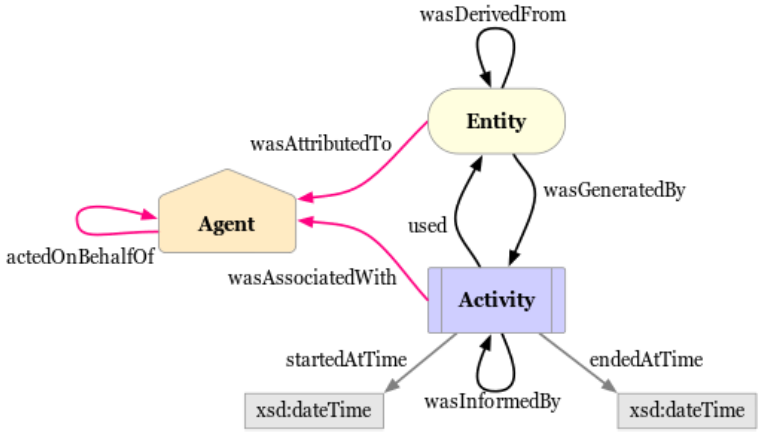
\includegraphics[scale=0.6]{prov}
	\caption{Overview of the main components of PROV-O \cite{733f89c65e4844f9aabcae1c276a5602}}
	\label{fig:prov} % \label has to be placed AFTER \caption (or \subcaption) to produce correct cross-references.
\end{figure}

In Figure \ref{fig:prov} there is the basic setup of the PROV-O concept. It consists of three main elements. The Entity is any physical, digital, conceptual thing. Provenance records describe Entities that can consist of references to other Entities. Another element is the Agent, which is responsible for Activities and that they are taking place, e.g. software, persons or organizations. The association of an Agent to an Activity defines the responsibility of the Agent for the Activity. An Activity describes what happened that the Entity has come to existence and how attributes of an Entity changed \cite{733f89c65e4844f9aabcae1c276a5602}. The representation of the context information is not specified in the design chapter \ref{Design}, therefore the PROV ontology can be used to represent the information. In this thesis the PROV-O standard is not implemented, since the EODC back end providers wanted their own representation of it, which is an extension of the existing meta-data, but since it is a reasonable extension it is mentioned in the future work Section \ref{FutureWork}.

\subsection{VFramework}

The basic concept of the VFramework is that the execution is done with parallel capturing of provenance data. During the original execution evidence gets collected into a repository e.g. logging of the needed meta-data. All of which is persisted in the context model of the execution e.g. a database record. A re-execution can then be verified and validated using the provided provenance data in the context model of the original execution and the context model of the re-execution. The provenance data is divided into static and dynamic data. Static data defined in the VFramework is data that is not dependent on the execution of the experiment e.g. the operating system and installed packages. The static environment information is therefore independent from the set up and the configuration of the execution. Dynamic data on the other hand has to be captured during the execution of the original experiment e.g. python version of the execution or used input files. It describes the data that is specific for one work-flow execution \cite{Miksa2013FrameworkFV}. 
In Figure \ref{fig:vframework} there is an overview of the VFramework concept.  
\begin{figure}[h]
	\centering
	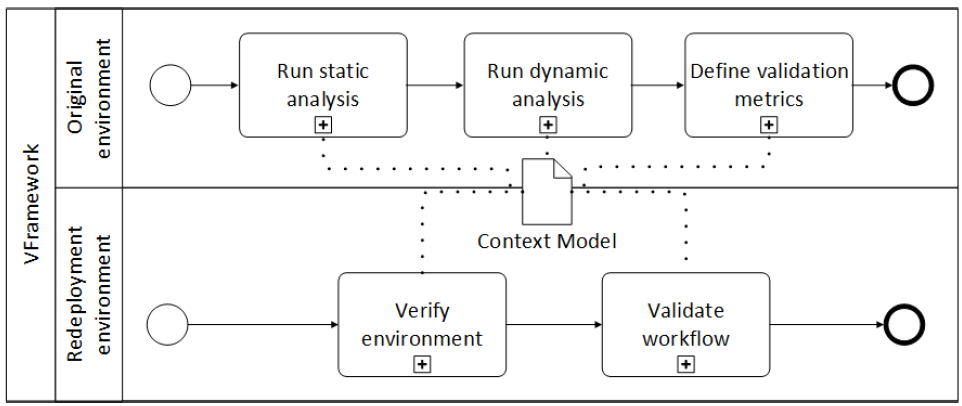
\includegraphics[width=\textwidth]{vframework}
	\caption{Overview of the Concept of the VFramework \cite{Miksa2013FrameworkFV}}
	\label{fig:vframework} % \label has to be placed AFTER \caption (or \subcaption) to produce correct cross-references.
\end{figure}


\section{Earth Observation Science}\label{EOScience}

Reproducibility is a well discussed topic of the computational geoscience. The high amount of earth observation data leads to complex research experiments and therefore high complexity in the papers.  In \cite{Ostermann2017AdvancingSW} reproducibility and replicability of scientific papers in geoscience are tested by obtaining more than 400 papers. In \cite{Ostermann2017AdvancingSW} a reproduction is defined by an exact duplicate of an experiment, whereas a replication is defined as a resemblance of the original execution, but allowing variation e.g. different scales. Table \ref{Tab:geoprimad} describes the difference of reproduction and replicability in PRIMAD terms. Only half of the test group publications are replicable and none of them reproducible. There are publications to address this lack of reproducibility in the earth observation science. The sections below summarize some examples of earth observation communities that are working on the topic of reproducibility.   

\begin{table}[]
	\caption{PRIMAD description of reproduction and replication according to \cite{Ostermann2017AdvancingSW}}
	\begin{tabular}{l|l|l}
		 & \textbf{Reproduction} & \textbf{Replication}  \\ \hline
		\textbf{P}latform & same & different \\ \hline 
		\textbf{R}esearch Objectives & same & same \\ \hline  
		\textbf{I}mplementation  & same & different  \\ \hline  
		\textbf{M}ethods & same & different \\ \hline 
		\textbf{A}ctors & different & different \\ \hline
		\textbf{D}ata & same & different, but similiar \\ \hline
	\end{tabular}
	\label{Tab:geoprimad}
\end{table}



\subsection{Vadose Zone Journal (VZJ)}\label{VZJ}
In order to face the issue of lacking reproducibility in geoscience the Vadose Zone Journal (VZJ) started a Reproducibility Research (RR) program in 2015 \cite{doi:10.2136/vzj2015.06.0088}. 
The earth observation science is a big part of VZJ publications and most of them are not applying the open computational science guidelines. The main reasons are behaviors of scientists that do not see the overall benefit of putting effort into documentation. Therefore, the VZJ started an RR program to publish alongside the scientific paper the code and data used by the scientists for evaluating the publication. This shall lower the access barrier for scientists to publish their research work entirely. Aim of the project is to create a community of researchers with a common sense of reproducibility and data citation on the platform and to animate other scientists to join the approach. On the time this thesis is written, the service is still available\footnote{https://dl.sciencesocieties.org/publications/vzj/author-instructions-reproducible-research}, but there were no results available on how much it is used \cite{doi:10.2136/vzj2015.06.0088}.

\subsection{The Geoscience Paper of the Future (GPF)}\label{GPF}

The geoscience paper of the future (GPF) is according to \cite{Gil2016TowardTG} a proposed standard to help geographical scientists by making reproducible publications. It defines recommendations on data management and software management, by introducing the reader to available repositories. The gain of it is applying concepts of open science and reproducibility to earth observation papers. A GPF needs to apply the following requirements:

\begin{itemize}
	\item \textbf{Reusable data} in a public repositories and persistent identifiers.
	\item \textbf{Reusable software} (including software for preparing and post editing of the data) in a  public repositories and persistent identifiers.
	\item \textbf{Documenting the computational provenance of results} in a public repositories and persistent identifiers.  
\end{itemize}

\begin{figure}[h]
	\centering
	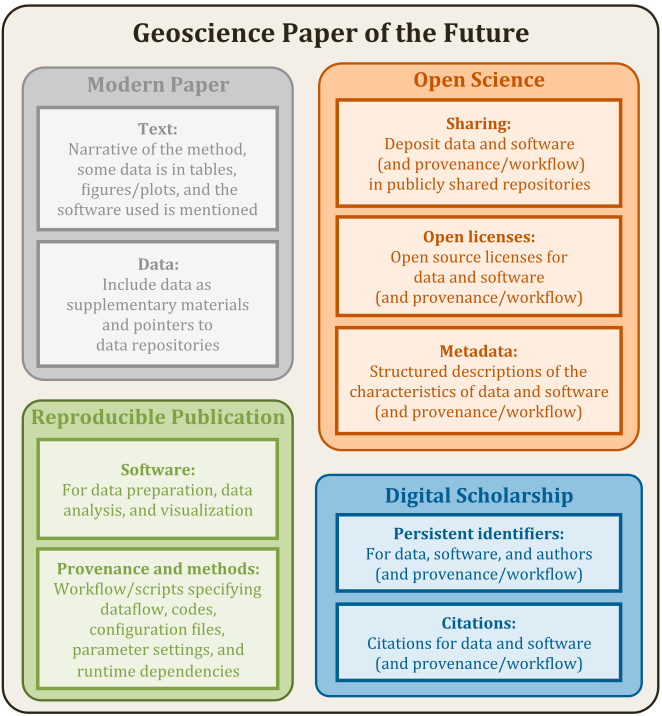
\includegraphics[scale=0.5]{gpf}
	\caption{Comparison between reproducible publications and geoscientific papers of the future \cite{Gil2016TowardTG}}
	\label{fig:gpf} % \label has to be placed AFTER \caption (or \subcaption) to produce correct cross-references.
\end{figure}

In Figure \ref{fig:gpf} the differences with a reproducible paper gets visualized. In addition to the characteristics of the reproducible paper the GPF focuses on publishing the data publicly with open licenses with citable persistent identifiers.
The GPF consists of a set of 20 recommendations for geoscientists regarding data accessibility, software accessibility and provenance information. GPF authors may find reasons to not be able to follow the rules and therefore have to find workarounds and propose areas for future improvements. The strategy of the GPF community is to educate the scientist to make reproducible publications, by making training sessions for them\footnote{http://scientificpaperofthefuture.org/gpf/events.html}, rather then providing tools to make it easier for scientists to use it. In comparison to this thesis it is a different approach to achieve the same goal, in this thesis the strategy is to achieve reproducibility in geoscience through technology. 

\subsection{Climate Change Centre Austria (CCCA)}

The Climate Change Centre Austria (CCCA) is a research network for Austrian climate research online available since 2016 and has 28 members. The main tasks are the provision of climate relevant information, the inter-operable interfaces and long term archiving of scientific data. In 2017 the NetCDF data citation was added to the project. The set up of the data service and the technology used in the background is similar to the set up of the EODC back end. Therefore, the process of enabling data identification was similar to this thesis. CCCA is Open-source and available at GitHub, see the GitHub repository\footnote{https://github.com/ccca-dc}. The concept used for gaining data citation was the RDA recommendations defined in \cite{rauber2016identification}. Figure \ref{fig:ccca} shows an overview of the CCCA implementation. It uses a ckan\footnote{https://ckan.org} webserver to handle the request and responses of the user, which are then passed to an python application. The python part is responsible for the query store functionality. The core element is the Thredds Data Server (TDS)\footnote{https://www.unidata.ucar.edu/software/thredds/current/tds/}, which is responsible for the actual data archive.   
The python application part of the CCCA overview is similiar to the implementation of this thesis. The main difference are the objectives of the CCCA service compared to the EODC back end. On the CCCA platform, any climate relevant information (e.g. air temperature or frost days) can be uploaded and persisted. On the EODC back end, preprocessed global earth observation data is persisted, which is used as input data for processing chains. Therefore, the data on EODC is more homogeneous than the data on the CCCA platform. Nevertheless, the concept of enabling data identification is similar in both projects. The basic query store implementation of this thesis was inspired by the CCCA implementation. The query result differs, because EODC uses GeoTiff instead of NetCDF at their back end. Another difference is that CCCA uses HTTP GET requests as query, whereas the EODC back end uses XML based queries, which are in addition limited by the OpenEO API specification  \cite{ccca}.  

\begin{figure}[h]
	\centering
	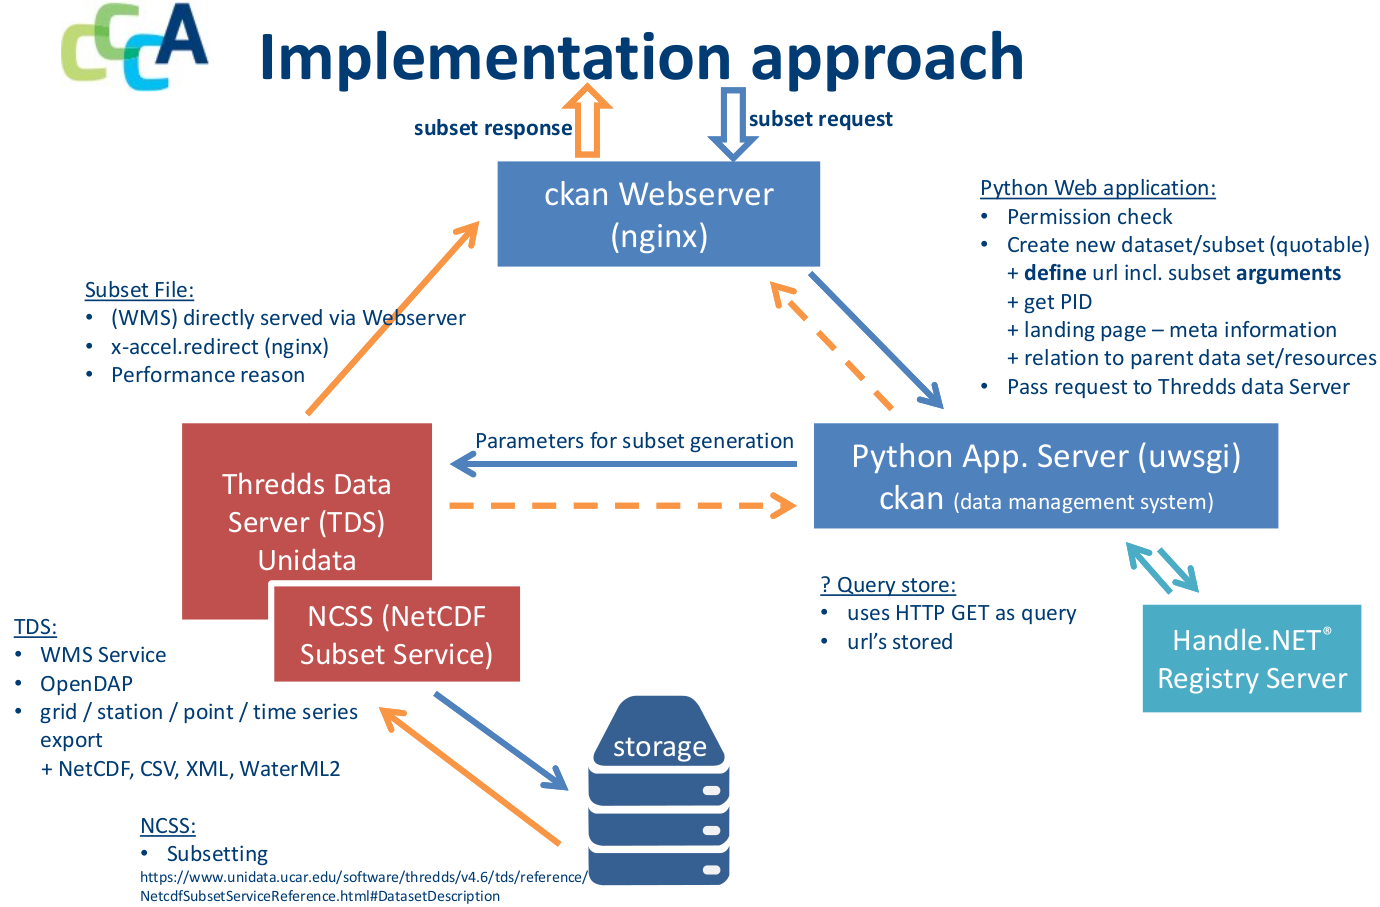
\includegraphics[scale=0.25]{ccca}
	\caption{Concept of the CCCA NetCDF Cata Citation}
	\label{fig:ccca} % \label has to be placed AFTER \caption (or \subcaption) to produce %correct cross-references.
\end{figure}

\section{Data Identification}\label{Data Identification}

Data identification and citation is a main concern in many computer relying sciences. For the aim of this work, the input data is a key element of the capturing. If the input data can not be identified correctly, the capturing of the processing on it does not gain useful information. Therefore the identity of the data has to be guaranteed. The Research Data Alliance (RDA) presents general solutions to achieve data identifications. There are 14 recommendations defined to achieve the identification of an exact version and subset of input data. The recommendations are independent of the type of data and database system. In the following the recommendations are summarized \cite{rauber2016identification}.


\begin{itemize}
	\item \textbf{R1: Data Versioning} \\
	Changes on a data record must result in a new version of the data record and the persistence of the deprecated data records. All data record versions have to be identifiable and accessible. 
	\item \textbf{R2: Timestamping} \\
	All changes to the database have to be comprehensible via timestamps. Every time changes are applied to the data, there has to be a time stamp persisted to describe when it happened. 
	\item \textbf{R3: Query Store Facilities} \\
	There has to be a query store implemented at the data provider to store queries including their meta-data, to be able to re-execute them in the future. The database has to store, according to \cite{rauber2016identification}, the following things: 
	\begin{itemize}
		\item The original query as applied to the database
		\item A potentially re-written unique query created by the system (R4, R5)
		\item Hash of the (unique) query to detect duplicate queries (R4)
		\item Hash of the result set (R6)
		\item Query execution time stamp (R7)
		\item Persistent identifier of the data source
		\item Persistent identifier for the query (R8)
		\item Other metadata (e.g. author or creator information) required by the landing page (R11)
	\end{itemize}
	\item \textbf{R4: Query Uniqueness} \\
	Since it is not desirable to have equal queries with the same result stored at the query store, there needs to be a normalized query that can be directly compared to other queries. Hence, there needs to be an algorithm to normalize the queries and to guarantee their uniqueness.
	\item \textbf{R5: Stable Sorting} \\
	The sorting of the resulting data has to be unambiguous if the sequence of data item presentation is essential for the reproduction.
	\item \textbf{R6: Result Set Verification} \\
	To ensure that the resulting data of the query is comparable there have to be a checksum or hash key of it. 
	\item \textbf{R7: Query Timestamping} \\
	There has to be a time stamp assigned to every query in the query store, which can be set to the latest update of the entire database, or the query dependent data of the database, or simply the time of query execution.
	\item \textbf{R8: Query PID}\\
	Every query record in the query store must have a Persistent Identifier (PID). There should not be a query with the same normalized query and the same query result checksum. 
	\item \textbf{R9: Store the Query} \\
	The data described in previous recommendations have to be persisted in the query store.
	\item \textbf{R10: Automated Citation Texts} \\
	To make the citation of the data more convenient for researchers, there shall be a automatic generation for the citation text snipped containing the query PID.
	\item \textbf{R11: Landing Page} \\
	The PID shall be resolvable in a human readable landing page, where data mentioned in the previous recommendations is provided to the scientist.
	\item \textbf{R12: Machine Actionability} \\
	Providing an API landing page so that not only humans, but machines can access the meta-data by resolving the PID.
	\item \textbf{R13: Technology Migration} \\
	If the database where the query store is implemented needs to be migrated to a new system, the queries need to be transferred too. In addition the queries have to be updated according to the new setup, so that they still work exactly like in the old system.
	\item \textbf{R14: Migration Verification} \\
	There shall be a service to verify a data and query migration (see R13) automatically, to prove that the queries in the query store are still correct. 
\end{itemize}
The implementation of the recommendations for the purpose of this thesis is described in Section \ref{Implementation:Data Identification}. 

\section{Tools for Reproducibility}\label{Existing Tools}
The section describes tools that are designed to solve similar problems or subproblems that are addressed by this thesis. There is an explanation why the specific tool was not used for the prototype of this thesis or how it was used in parts of the solution. 

\subsection{noWorkflow}\label{Noworkflow}
noWorkflow is introduced in \cite{c9e0604becba42af96a9cb0a6f60018b} as a script provenance capturing tool with the aim to not influence the way researchers implement experiments. As proof of concept the noWorkflow command line tool got implemented for python. The provenance is captured in a SQLite database by different trials. A trial represents the environment information of one execution.The main benefit of noWorkflow is that it does not instrument the code and it automatically captures the definition, deployment and execution environment in a local SQLite database. The stored meta-data can be accessed via the command line interface of noWorkflow. In addition to just retrieving the information about the execution environment, analyses features are added \cite{c9e0604becba42af96a9cb0a6f60018b}.

\begin{figure}[h]
	\centering
	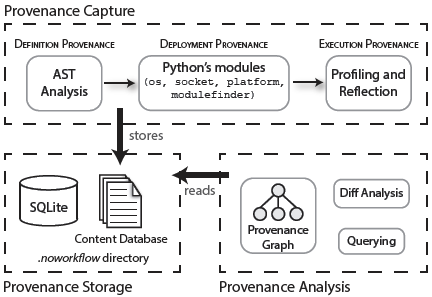
\includegraphics[scale=1]{noworkflow}
	\caption{Architecture of noWorkflow \cite{c9e0604becba42af96a9cb0a6f60018b}}
	\label{fig:noworkflow} % \label has to be placed AFTER \caption (or \subcaption) to produce correct cross-references.
\end{figure}

The noWorkflow framework got improved regularly after the first announcement. In \cite{Pimentel2016TrackingAA} an additional feature of tracking the evolution of the experiment execution is added. It improves the possibility to compare different trials of an experiment and to visualize the history of past executions. In \cite{Pimentel:2016:FPC:3090188.3090214} the fine-grained provenance tracking extension of noWorkflow is introduced. With it the execution of the python script can be viewed as a set of execution lines. It adds a visualization of all called functions with the exclusion of calls in one line on complex data structures such as dictionaries, lists and objects. In \cite{69bac1252a684629baa43b48e350068d} the provenance capturing of noWorkflow in combination of yesWorkflow, which gathers information about the provenance using comments and annotations (see \cite{192094}), got combined. The combination enabled a more detailed environment information, querying and visualizations. 
In this thesis noWorkflow is used in an alternative attempt of the implementation described in Section \ref{Implementation:Noworkflow Implementation}, but is not part of the final solution due to reasons provided in Section \ref{Evaluation:NvsP}.

\subsection{ReproZip}\label{ReproZip}
ReproZip is a packaging tool to enable the reproducibility of computational executions of any kind. It automatically tracks the dependencies of an experiment and saves it to a package that can be executed on another machine by ReproZip. It is even capable of letting the re-executor modify the original experiment. It was developed for the SIGMOD Reproducibility Review. In Figure \ref{fig:reprozip} the architecture of ReproZip is shown in detail. It traces the system calls to create a package defined in the configuration file. Thus, a single file with the extension “.rpz” gets produced. These type of files can then be unpacked on a different machine and re-executed. The aim of ReproZip is to make reproducible science easy to apply for single experiments \cite{29c5846926a4497d95f276604cb0368c}. The reason why it is not used in the solution of this thesis, is that the capturing is very fine granulated and takes too much performance from the back ends, which is a key selling point for back end providers. Depending on the back end, the payment for users may be dependent on the duration time of the processing. Another issue with ReproZip in the context of this thesis is that it is not capable of capturing the big data of the back ends within the package, because it would take too much space and performance.  

\begin{figure}[h]
	\centering
	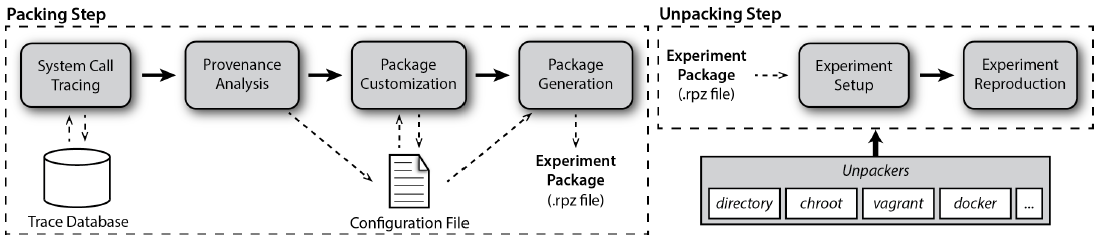
\includegraphics[width=\textwidth]{reprozip}
	\caption{Overview of the ReproZip concept from \cite{29c5846926a4497d95f276604cb0368c} }
	\label{fig:reprozip} % \label has to be placed AFTER \caption (or \subcaption) to produce correct cross-references.
\end{figure}

\subsection{Docker / Smartcontainer}\label{Smartcontainer}
Docker containers are very common in geoscience executions. The advantages on reproducible research and cost savings by using docker containers is discussed in \cite{rs9030290} for the Geographic Object-Based Image Analysis (GEOBIA). The docker implementation of the image analysis was implemented with a docker image including a user interface that can be used by non-experts. There are experiments for the more general Object-Based Image Analysis (OBIA) with docker containers presented in \cite{proceedings456}. The conclusion of the previous mentioned paper is very positive with only little shortcomings in the usability. The two papers mentioned above are using the docker images to make it easy to re-run an experiment on the OBIA system. Remaining question is how the docker configuration can be preserved in a manner so that it can be reproduced in different environments. The aim of \cite{emsley2017a} is to answer this question by introducing, in addition to the Docker description file, a workflow record saving the environment and entities involved. A SPARQL query got introduced to create the possibility to use the container as a repository of metadata.\\ 
Another approach of preserving a docker container are smart container introduced in \cite{Huo2015SmartCA}. The aim of smart container is an ontology and software to preserve docker metadata. It uses the PROV-O standard to define the provenance. 
Docker containers are used at the EODC back end for running all services, therefore they are part of the solution. The description files of the used docker containers are persisted in the GitHub repository of the EODC back end, hence they are identifiable by the back end version defined in Section \ref{Design}.   


\subsection{Version Control Systems}\label{Version Control Systems}
Version control systems (VCS) became a very important part in all computational sciences. It enables to persist versions of code and the possibility to head back to a certain version of it. Before that programmers tend to have multiple directories to version the code. The basic idea of VCS is that via a command line interface it is possible to set a version of the current state of the code. These versions can be accessed in future, without changing other versions of the code and without multiple folders \cite{10.1109/MCSE.2009.194}. 
In this thesis Gitorious (Git) is used as version control system. Versions in git are defined as commits and are stored locally, but can be published to an external server, where, depending on the user rights, they are accessible for other users. The commits are stored locally and remotely \cite{QuickGit}. In example OpenEO uses Git as code version tool and GitHub is used as the publicly available server. Since OpenEO is an open source project, the code of every back end, core API and client is available at GitHub.  

\subsection{Hash}\label{Hash}
Hash functions are used to validate the data without having to save the whole data. They have three important properties to work properly. First the probability that two different inputs have the same hash outcome has to be low. Second it needs to be hard to find a message with the same hash value as an already known message. The properties described above makes the hash functionality a common tool to identify data without having to save the original one \cite{3b412889270f46f59740fbf1ca8cd7e0}.  
There are different hash functions available. In this thesis the SHA-256 is used for the meta-data of the context model, mostly to compare differences in data outcomes.

%\begin{figure}[h]
%	\centering
%	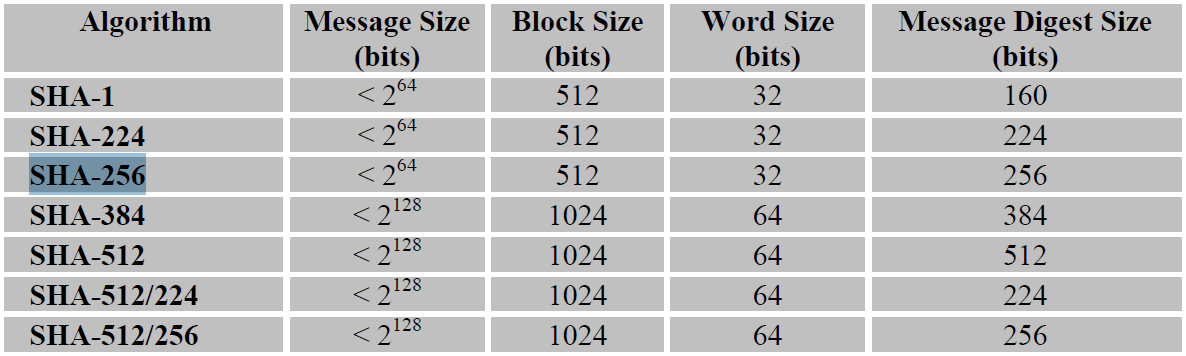
\includegraphics[width=\textwidth]{sha}
%	\caption{\cite{shapaper}}
%	\label{fig:sha} % \label has to be placed AFTER \caption (or %\subcaption) to produce correct cross-references.
%\end{figure}
%The SHA-256 is chosen in the implementation, because of the best combination of performance and security of the above described properties of the hash. 



\section{OpenEO}\label{OpenEO}
The OpenEO project consists of three modules, the client module written in the programming language of the users, the back end drivers that enables for every back end to understand the calls from the clients and the core API that specifies how the communication takes place. The core API is a standard that the back end providers accepted to implement on their systems. The back end drivers are the translation of the client calls to the back end specific API. This architecture decouples the clients from the back ends so that every client can connect to every back end that complies with the OpenEO core API standard see Figure \ref{fig:api2} . An example of a workflow would be the example defined in Section \ref{example} that a scientist wants to run on the EODC back end and defines the processing with the python client in python code \cite{openeo}.  

\begin{figure}[h]
	\centering
	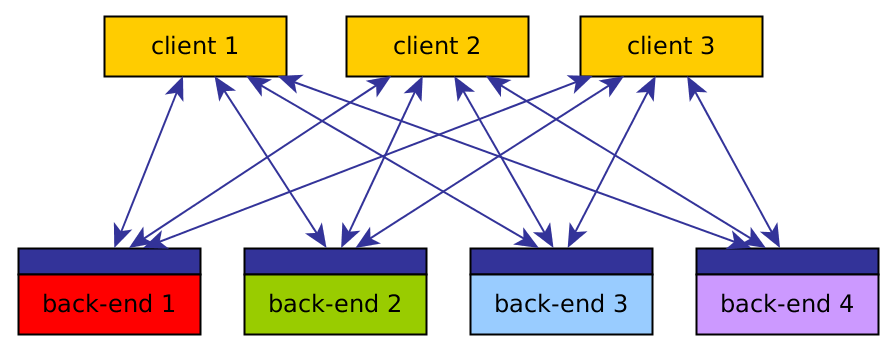
\includegraphics[width=\textwidth]{api2}
	\caption{Overview of the OpenEO architecture}
	\label{fig:api2} % \label has to be placed AFTER \caption (or \subcaption) to produce correct cross-references.
\end{figure}


The communication is specified as an OpenAPI description, which is a way of defining RESTful communication in a standardized way. The definition consists of the end points at the back end and the requests and the responses. The whole communication protocol is specified with OpenAPI \cite{openapi}. 
In the following the relevant RESTful request types in OpenEO and the policy of choosing between them are introduced.

\begin{itemize}
	\item \textbf{GET Request} \\
	GET requests are used to retrieve data and meta-data from the back ends. The functionality is limited to read operations on the data records. \\(e.g. GET /collections returns a list of available collections at the back end.)
	\item \textbf{POST Request} \\ 
	POST requests are used to create new data and meta-data records at the back end. It is also used to carry information to the back end.  \\(e.g. POST /jobs creates a new processing job at the back end, which is defined in the body of the request.)  
	\item \textbf{PATCH Request} \\
	PATCH requests are used to update an existing record at the back end. \\(e.g. /PATCH /job/{job\_id} modifies an existing job at the back-end but maintains the identifier.)
	\item \textbf{DELETE Request} \\ 
	DELETE requests are used to remove existing records from the back end. \\(e.g. /DELETE /job/{job\_id} removes an existing job from the back end.)
\end{itemize}

\subsection{Job Execution}\label{Job Execution}
The job execution workflow in OpenEO starts at a client application that lets the user define what has to be processed in the client specific programming language.
The main part of the job execution definition is based on the description of what input data shall be used, which filters have to be applied and the processes that should be executed on the data. Therefore, OpenEO introduces the process graph, which is defined as a tree structure describing the processes with their data and the input data identifier. The input data id is back end specific. The process graph has a JSON format and gets generated by the clients in the background without users noticing it directly. In Figure \ref{fig:process_graph} there is an example of a process graph. 

\begin{figure}[h]
	\centering
	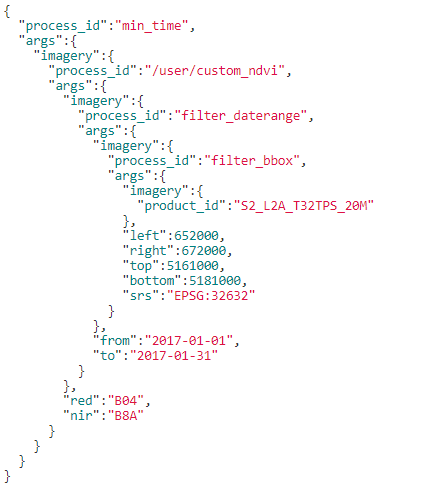
\includegraphics[scale=1]{process_graph}
	\caption{Process graph of the running example defined in Section \ref{example}}
	\label{fig:process_graph} % \label has to be placed AFTER \caption (or \subcaption) to produce correct cross-references.
\end{figure}

The back ends interpret the process graph from inside out. Figure \ref{fig:process_graph} displays the process graph of the running example of Section \ref{example}. It describes the calculation of the minimum NDVI image of the Sentinel 2 satellite over south tyrol in May 2017. The element in the center of the process graph defines the input data identifier in the "imagery" block, with the "get\_collection" process id. In this case the "s2a\_prd\_msil1c" is chosen as input data identifier, because it is the identifier for Sentinel 2 at the EODC back end. After reading the input data id, the back end iterates one step up in the hierarchy of the process graph and calls the process "filter\_bbox" with the parameters "left", "right" and so on, which is responsible of filtering the image spatial (e.g. the area over south tyrol). After that the "filter\_daterange" process is used to only take imageries from May 2017. Every process beginning with "filter\_" is a filter operation that specifies the selection of the input data. The output data of the previous process is the input data of the next process. After the last filtering process, the NDVI gets called by "/user/custom\_ndvi" with the parameters "red" and "nir", which take the identifier of the bands of near infrared and red light, which is needed by the NDVI process (see Section \ref{example}). After that the minimum value is taken from all images using the "min\_time" process, which then results in a single image. In Figure \ref{fig:process_graph_diagram} the same process graph is visualized from the back end point of view, visualizing the order of how it gets executed. To transfer the process graph in Figure \ref{fig:process_graph} at a back end, it gets sent in the body of the POST /jobs endpoint request.

\begin{figure}[h]
	\centering
	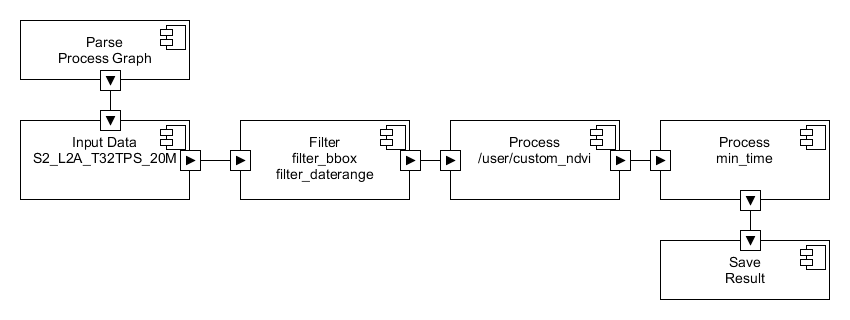
\includegraphics[width=\textwidth]{backend_pg}
	\caption{Action chain of the back end after receiving the process graph of Figure \ref{fig:process_graph}}
	\label{fig:process_graph_diagram} % \label has to be placed AFTER \caption (or \subcaption) to produce correct cross-references.
\end{figure}

There are two different kinds of process executions depending on the back ends capabilities, synchronous and asynchronous calls. Synchronous calls are directly executed after the back end receives them and the user has to wait until the job is finished. For example on the python client the program waits after sending the process graph to the back end until the back end returns the result, which is directly returned to the user. An asynchronous call does not get executed until the user starts the execution on the back end through an additional endpoint call. When the processing is finished the user can download the result at another endpoint of the back end. For asynchronous calls there is the possibility to subscribe to a notification system on the back end, so that the user gets notified when the job execution finished.     
The processes are defined at the OpenEO core API and therefore independent of the back end they get called at, other than the data identifier, which is different for every back end.  
\\
The previous example uses a process graph that only consists of the available processes and data of the back end. Within the OpenEO\footnote{https://github.com/Open-EO/openeo-openshift-driver/tree/release-0.0.2} project there is the possibility to define individual processes and execute them on the back end. In the project they are called “user defined functions” and are at the writing of this thesis still not well-defined, but are basically code written by the OpenEO user that gets sent to the back end and executed there at a secure environment. The user can define processes and can run them with the data provided at the back end, using the infrastructure of the back end. Every back end has to individually define what the restrictions on user defined functions are. 

\subsection{Back end Overview}\label{Back end Overview}
Even though the back ends implement the OpenEO core API standard, they are still diverse behind this abstraction layer. Some back ends have already an API, where the OpenEO calls have to be adapted to. There are 7 partners within the OpenEO project that are implementing a back end driver. The back ends have to manage the translation of the process graph to the actual code that executes the defined process chain. The billing of the users can be completely different on every back end. In Table \ref{Tab:backends} there is an overview of all contributing OpenEO back ends and the related GitHub repository. 
\begin{table}[]
	\caption{List of all back end providers of the OpenEO project}
	\begin{tabular}{l|l}
		\textbf{Organisation} & \textbf{GitHub}  \\ \hline
		EODC & \url{https://github.com/Open-EO/openeo-openshift-driver} \\ \hline 
		VITO & \url{https://github.com/Open-EO/openeo-geopyspark-driver} \\ \hline  
		Google  & \url{https://github.com/Open-EO/openeo-earthengine-driver} \\ \hline  
		Mundialis & \url{https://github.com/Open-EO/openeo-grassgis-driver} \\ \hline 
		JRC & \url{https://github.com/Open-EO/openeo-jeodpp-driver} \\ \hline
		WWU & \url{https://github.com/Open-EO/openeo-r-backend} \\ \hline
		Sinergise & \url{https://github.com/Open-EO/openeo-sentinelhub-driver} \\ \hline
		EURAC & \url{https://github.com/Open-EO/openeo-wcps-driver} \\ 
	\end{tabular}
	\label{Tab:backends}
\end{table}

\subsection{EODC Back End}\label{EODC Back End}

The EODC back end is one of the contributing back end providers of the OpenEO project. It is in general a python implemented back end that uses virtualisation technologies for the job execution. The overlaying technology is OpenShift (using Kubernetes) \footnote{https://www.openshift.com/learn/what-is-openshift/}, which is capable of scaling docker containers and handles the execution of them. In the docker containers the python code for the processing gets executed. The docker description files and the python code is available on GitHub. In this thesis the latest version of the EODC back end provided in GitHub with the version 0.3.1 is used. In this version every process of the OpenEO process graph is represented by an own docker container running the python code needed. The service layer for accessing the back end is accomplished by the python library Flask. EODC provides only data from Sentinel 2 and Sentinel 1 within the OpenEO project. The provided data are satellite images from the European Space Agency (ESA), which gets the raw data coming directly from the Sentinel satellites. \\
The data management of EODC is file-based, so every image data is stored in a unique directory and filename combination. Meta-data is provided via PostgreSQL database including the PostGIS\footnote{https://postgis.net} plug-in. The provided query tool for EODC users is the Open Geospatial Consortium (OGC) standard interface Catalogue Service for the Web (CSW\footnote{http://cite.opengeospatial.org/pub/cite/files/edu/cat/text/main.html}). In Figure \ref{fig:eodceer} an overview of the EODC meta-database is displayed. The structure is retrieved from the github repository of the EODC back end\footnote{https://github.com/Open-EO/openeo-openshift-driver}, where every database entity is defined. Every Process entity can have parameters described by the Parameter entity. The ProcessNode is representing one node in a process graph and is therefore related to exactly one ProcessGraph entity. Every Job has a related process graph, there may be jobs that use the same process graph, but in the current set up they are persisted both in the database.

\begin{figure}[h]
	\centering
	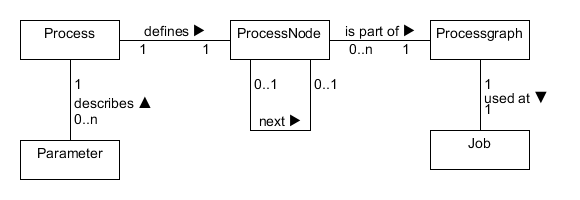
\includegraphics[width=\textwidth]{eodc_eer}
	\caption{Overview of the EODC meta-database structure.}
	\label{fig:eodceer} % \label has to be placed AFTER \caption (or \subcaption) to produce correct cross-references.
\end{figure}

\section{Summary}

For the research areas that are related to the solution of the thesis a vast amount of literature is available. The problem description of the thesis has many possible solutions described in this chapter. The outcome of this thesis has the aim of making it easy for the scientists to reproduce experiments, other than presented solutions for earth observation science like the VZJ approach or the GPF, which tries to motivate scientists to do it themselves. The implementation of Section \ref{Implementation} builds on existing systems like the implementation of the CCCA query store. The following chapter describes the design of the solution. 




 
\chapter{Design}\label{Design}
This chapter describes the concept of capturing the environment of a geoscientific experiment. The aim of this chapter is to explain the general concept of how to gain reproducibility in an earth observation environment. It is structured in six parts. The first part presents an overview of the concept. The next three sections describe the main components of the overview in detail, first the data identification part, then the back end provenance and the job dependent provenance. The following section defines the resulting context model. The next section of this chapter defines the user interfaces needed to use the data of the context model from an earth observation scientist's perspective. The last section gives an overview of the capturing of User Defined Functions (UDF). The following Chapter \ref{Implementation} shows an implementation of the concept of this chapter at the EODC back end. 



\section{Overview}\label{Design:Overview}
This section presents an overview of the concept and in Figure \ref{fig:overview} it is visualized. The components that every back end driver has in place are represented by the white boxes. The green elements in Figure \ref{fig:overview} are the proposed extensions of this design. The typical job execution work-flow is described in the following steps:

\begin{figure}[h]
	\centering
	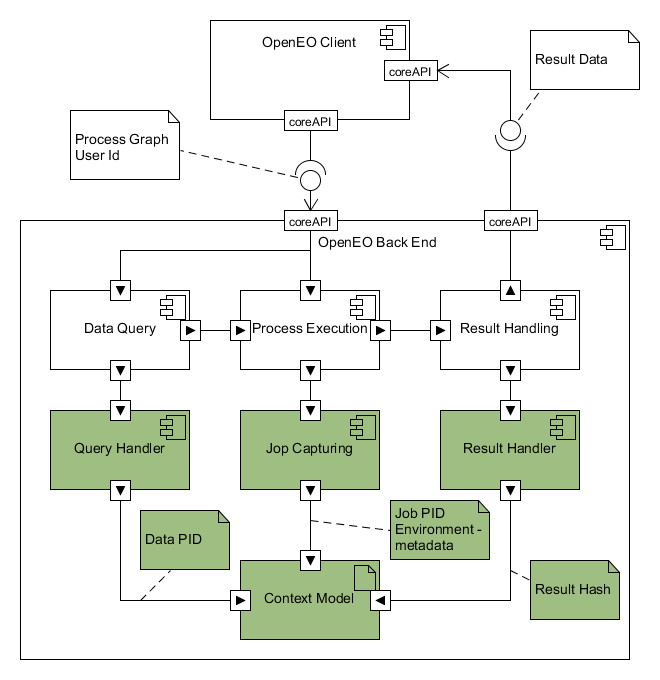
\includegraphics[scale=0.6]{design_overview}
	\caption{Overview of the Design}
	\label{fig:overview} 
\end{figure}

 \begin{enumerate}
	\item \textbf{EO Client} \\
	The user defines the input data, the filter operations and the processes that need to be executed at the back end via an earth observation client. Then the user orders the job to be executed, therefore the client creates a process graph description. The user identification and the process graph is sent via a RESTful endpoint defined by the back end driver interface (e.g. OpenEO).  
	\item \textbf{Data Query} \\ 
	The Data Query component receives the process graph and parses the data identifier and the filter operations out of it to query for the input data records needed for the job. These are forwarded to the Process Execution component.  
	\item \textbf{Process Execution} \\
	The Process Execution component receives the process graph and the input data from the Data Query component. It parses the processes from the process graph and executes them in the order of appearance. After every process defined in the process graph got executed, the Process Execution component forwards the resulting data to the Result Handling component.   
	\item \textbf{Result Handling} \\ 
	The Result Handling component receives the results from the Process Execution component and persists all meta-data about the job and the result. In the meantime the resulting data is sent back to the client application, if the job is not defined as a batch job. If it is a batch job the user has to actively order the results from the back end.  
\end{enumerate}

To make the whole workflow reproducible, every single component have to be identifiable. Hence, the following elements get introduced as additions to the back end.

 \begin{itemize}
	\item \textbf{Query Handler} \\
	The Query Handler component is responsible for applying data identification to the back end. The query has to be persisted and the resulting data generated by the Data Query component has to be identifiable by a PID. Section \ref{Design:Data Identification} describes the Query Handler in more detail.     
	\item \textbf{Job Capturing} \\ 
	The Job Capturing component is responsible for enabling code identification of the used software at the back end. Therefore, a PID of the code used for the processing has to be introduced. In addition, meta-data of the job execution environment gets captured, to gain feedback information for the users and capture the environment of the execution. Section \ref{Design:Job Capturing} describes the Job Capturing component in more detail.
	\item \textbf{Result Handler} \\
	The Result Handler component is responsible for creating a comparable result checksum or hash. The data created by an earth observation back end might be too big to be persisted, hence there need to be a checksum or hash to be capable of confirming equal results. Section \ref{Design:Result Handler} describes the Result Handler component in more detail.   
	\item \textbf{Context Model} \\ 
	The Context Model is not a component, but a data set that contains all the meta-data mention in the previous components. One context model is related to one job execution. Section \ref{Design:Context Model} provides more detailed information about the Context Model. 
\end{itemize}

\section{Query Handler}\label{Design:Data Identification}
The input data of the processing is crucial for the outcome of the job execution. Even though the process graph already contains an identifier of the input data, unique for the specific back end, internal changes to the data set might not result in a new identifier. So jobs called later in time might use another version of the input data than the previous jobs. To prevent this the input data has to be persisted according to the 14 steps of data provenance defined by the RDA \cite{rauber2016identification}. Every back end is responsible for applying data identification. It is assumed that the back ends preserve the data as described in Section \ref{Design:Data Identification}. The Query Handler is the module where the data persistence is implemented and depends highly on the structure and architecture of the back end. Therefore, no common definitions can be made for all back ends in this section. In Chapter \ref{Implementation} there is a fully implemented solution at the EODC back end. The context model elements of the job executions are specified with a "J" in the beginning for readability reasons. Elements of context model related to the back end environment are specified with a "B" in the beginning. Each element represents one data entry of the resulting context model. The input data is represented in the context model by the following element: \\
\\
\textbf{J1: Input data persistent identifier} \\
The output of the Query Handler is the PID of the input data related to a job execution. Every job execution uses input data, which has a PID assigned to it. Therefore, the PID is added to the job dependent context model. 

\section{Job Capturing}\label{Design:Job Capturing}
The aim of this section is to describe the job execution capturing and a description of data that shall be captured. The meta-data provided by the job capturing can be categorized in static and dynamic data, where static data is defined as not dependent on job properties and dynamic data is defined as job dependent information. In the following two sections the static data (in this thesis called back end provenance) and dynamic data (in this thesis called job dependent provenance) are further described.     

\subsection{Back end provenance}\label{Design:Back end provenance}
The scope of this part of the context model is to get the static environment of where the job execution at the back end takes place. It contains the provenance data that is independent of a job execution, so it does not change through job executions, regardless of how many jobs were processed. It can only change from inside of the back end by their maintainers. The earth observation community has a great variety of different back end providers with very distinct setups. The challenge of this part of the design is to make it simple and generic. Data captured in this part of the context model is not meant to be shown to the user directly, because of security issues.  The context model elements of the back end environment are specified with a "B" in the beginning for readability reasons. Elements of the job dependent context model are specified with a "J" in the beginning. The following meta-data is suggested for the back end provenance:
\\ \\
\textbf{B1: Code identification} \\
Every earth observation back end has to provide an identifier for the used code. Therefore, a version control system has to be applied to the running services. If back end is open source, it can provide a GitHub repository were the used code is stored and publicly available. The aim of this strategy is to get other back ends with similar settings to reuse the already working setups of the running back ends. In this case the information is added to the back end provenance by saving the git repository URL, the used commit identifier and local changes to the repository. If the back end is not open source a local or secure version control repository has to be implemented to keep track of the different code versions. 
%\\ \\
%\textbf{B2: Used Folders} \\
%The back end will most probably not only use the GitHub repository for the processing, so that other folders are involved. For example configuration files may not be persisted in GitHub for security reasons. This information is also crucial for the job execution and therefore needs to be stored. Changes of this directory have to be detected and stored in the context model. Therefore, a checksum or hash key of the additional folders are created and persisted in the context model.     
%\\ \\
%\textbf{B3: OS and packages} \\
%The operating system can also have an impact on the processing and so it has to be stored to the context model too. Not only the information about the operating system, but also the installed packages are added to the context model. If the whole processing is done in a virtual container the operating system of that container shall be stored. If the whole processing is done in a docker container, the docker description file can be used for the environment data. 
\\ \\
\textbf{B2: API version} \\
The back ends API version is the version of the interface API it currently is using. The same API calls can resolve in different results if the version of it differs, hence the API version is persisted in the context model. 
\\ \\
\textbf{B3: Back end version} \\
The back end version is an identifier that gets updated on every change of the back end. This includes changes on the hardware and software, so that every change on the code identifier or the API version results in a new back end version.   
\\
To provide long term stability of the capturing, it is essential to implement a tool to automatically capture the environment data and persist it in a separate back end version store. Every change on any of the previously described back end meta-data has to be detected automatically and have to result in a new back end version.  
\\ \\
\textbf{B4: Publication time-stamp} \\
The time-stamp of when the version was accessible at the back end. The time-stamp stands for the beginning of the version of the back end. If there exists no time-stamp after that, then it is the current used version. This enables the possibility to find the version of the back end used by a job executed in the past, by only knowing the time it was executed.     

\subsection{Job dependent environment}\label{Design:Job dependent provenance}
This section describes the job dependent provenance of the context model. The data captured is tied to a specific job execution, so for every job a new context model gets created. The process graph is already a description of the processes that run at the back end. So sending the same process graph to the same back end again shall result in the same outcome. To assure that the process graph can be re-executed in the same way as the original execution, meta-data about the original execution gets captured. 
The following subsections describe the single elements of the context model in more detail. 

\subsubsection{Process Environment}\label{Job:Process Data}
This section describes the capturing of the process itself. As mentioned above the incoming process graph describes the process, but to be certain that the same process id results in the same code, the code version has to be added to the context model. To be able to identify code from different versions a source control management needs to be installed. An example of doing so is persisting the back end source code on a public platform like GitHub. The entry in the context model related to this was mentioned in Section \ref{Design:Back end provenance}.  \\
The way of executing a specific process graph is not only related to the code running it, but also by the dependencies of the code. Therefore, the programming language version and the additional used libraries of it are persisted in the context model. To gain more meta-information about the processing the start time and end time can be added to the context model via timestamps. This leads to the following capturing elements in the job context model.

\textbf{J3: Programming language}\\
The programming language of the code that is used for the processing. In addition the version of the programming language has to be included in this information.

\textbf{J4: Installed packages of the programming language}\\
To identify the environment of the code execution, the installed packages of the programming language shall be captured and added to the context model. The version of the packages have a high influence on the outcome, hence can be included in the context model. For example in python the installed modules are added with their versions to the context model. The information stored in this element is related to the job execution, because it depends on the work-flow of the execution, how the environment is configured, since the job execution may be done in a dynamically generated container.

\textbf{J5: Start and end time of process execution}\\
On the beginning of the process execution and at the end of it, a time-stamp is created. These timestamps are persisted in the context model.

\subsubsection{Back end provenance}\label{Job:Back end provenance}
The back end provenance described in Section \ref{Design:Back end provenance} defines the version of the code that is executed and therefore has to be added to the job context model. Over time the back end provenance will get updated so that every job need to persist a reference to the original back end configuration at the execution time. There are two solutions to achieve this. First the identifier of a specific version of the back end gets added to the context model. In this case the data of the back end environment versions have to be persisted and accessible. The second solution is to put a time-stamp of the execution into the job execution context model.

\textbf{J2: Back end provenance / code identifier} \\
The version of the back end provenance during the job execution. Since for every change on the back end a new version will be applied, the version of the back end is used as a code identifier for the execution. Another solution is to persist an execution time-stamp, so that the version of the given time can be identified.


\section{Result Handler}\label{Design:Result Handler}
The output data of the processing has to be captured as well to be able to compare job execution outcomes. In earth observation tasks the results can be rather big, that is why a simple generated hash value of the output result is enough. The output data does not have to be identifiable within the scope of this thesis, but just checkable of identity with other executions. Therefore, a generated hash value of the output data is sufficient. The aim of the output data capturing is not to add the possibility to find differences between results, but to be able to see that the results are different. Even though the input data of typical earth observation experiments are big, the output of such experiments are images of various sizes.   

\textbf{J6: Result hash} \\
The output result of the job need to be verifiable and therefore need to be persisted. An easy way to achieve this is to take the hash value over the output files sorted by the alphabetical ascending filenames.
 
\section{Context Model}\label{Design:Context Model}

The context model is the data record that saves the provenance of a job execution. The type of storage it is persisted in,  is defined by the infrastructure of the back end provider. It can be stored in a relational database or in a file-based system as a file on the file system. It has to be added to the meta-data database of the back end. The back end has to persist two different types of datasets: \\
First the back end environment dataset that saves job independent provenance and results in a back end version. The mandatory element of the back end environment is the back end version that defines the state of the back end in a specific time. The back end version need to be resolvable by a specific code version that was present in a past execution. In addition meta-data about the back end can be added. The elements (B1-B4) defined in Section \ref{Design:Back end provenance} are the suggestions of elements in the back end environment context model.\\
Second the job execution context model that includes all information that is dedicated to a specific job is persisted in the context model. There are three mandatory elements in the job context model. The input data identifier has to be persisted in the context model, so that it can be identified and used in future job executions. The used version of the back end related to the execution has to be included in the context model, to be able to re-execute it with the same code in the future. The output hash has to be added to the job dependent context model, so that different results can be detected. In Section \ref{Design} the elements (J1-J6) are additional job specific meta-data for the context model.  


%\textbf{J2: Process Code Identifier}
%The executed  code for the process has to be identifiable, therefore there has to be an id of the code. The OpenEO project is an OpenSource project and the back end provider have the used code at the Github repository, so the link to the github repository with the currently checked out commit can be used as the identifier. 

\section{User Services}\label{Design:User Interface}

In this section the information for the users and how it is provided gets described. The capturing described in the previous sections consists of information about the back ends that shall not be completely passed to the users in detail. For example, it is maybe a security risk to provide information on specific programming language packages. On the other hand the users need to be able to see the differences of job executions and get environment information about the back ends. Therefore, there has to be a filter on which data can not be shown to the users. Every captured information is not necessarily interesting for the users. Data that is not secure to the user has to be defined by the different back ends themselves. The earth observation community has a very diverse set of back ends and every one has a unique company security guideline.\\ 
Provenance information need be provided to the user. Therefore, there have to be additions to the core API specification. Additional endpoints for the users to get information about the back end have to be created for the core API, back end and client. The following recommendations summarize the set of needed additions, they are structured with a "U" in the beginning to add readability through the thesis. Other than the "J" and the "B" data elements, the following points are implementation recommendations for back end provider to make the use of the context model accessible for the users.

\textbf{U1: Back end version} \\
There has to be an endpoint for users to retrieve back end specific information especially the current version. The aim of it is to present the users with information about the current state of the back end and to help users to decide, which back end they want to use. 

\textbf{U2: Detailed Job Information} \\
The back end has to provide an endpoint to retrieve information about an already executed job. The provenance of the job has to be presented in there. At least the resolvable persisted identifier of the input data, the back end version and the result set hash has to be added to the view. In addition to this the whole meta-data of the context model can be made accessible. To make it more transparent for users the resolvable identifier URL of the input data and the GitHub information can be provided.   

\textbf{U3: Comparing Two Jobs} \\
The API has to add an end point for providing a comparison of two different jobs.  Every item of both of the context models of both jobs have to be compared if they are equal or not. Therefore, the response of the comparison request consists of the differences in the context model between two jobs.

\textbf{U4: Data Identifier Landing Page} \\
After the job is executed the input data has a relating input data PID. The PID has to be resolved by a landing page. The landing page provides the user with information about the input dataset and the query gets re-executed to view the concrete input data files upon request and given sufficient permissions.
    
\textbf{U5: Re-use of Input Data} \\
 The back end has to provide an endpoint to the user to re-use a specific input data in another job. Therefore, the API allows to include the use of an input data PID in the process graph, so that users can include cited data directly in a new created job description.  

\section{User Defined Functions}\label{Design:User Defined Functions}
This section describes a possible capturing method of User Defined Functions (UDF). UDFs are customized code written by the user that gets executed in a virtualization environment at the back end provider. In theory the user defines a docker base image and the code that should run in it. This is a black box for the back end provider, since they can not now what processes run in the docker container. Therefore, the capturing concept needs to be different then the common way of executing jobs at the back end. The code and the docker base image has to be persisted by the back end provider. In addition the timestamp of the execution, to be able to identify the back end version at the execution. This is a rather new concept in earth observation science and not implemented in the EODC back end, hence the implementation of the capturing is not part of this thesis.


\section{Summary}
This chapter presented the concept of the proposed solution system. The data elements needed to be able to reproduce a job execution are presented and described. To achieve it the data identification has to be implemented according to the RDA recommendations. The back end provenance got defined by the identification of the software and the version of the back end. The job dependent environment describes the environment of the job execution information and the result hash. The meta-data of the job execution got summarized into the context model. It consists of the data needed to answer the research questions of Chapter \ref{Introduction} In addition to the data description, the needed user interfaces to provide the functionality for the users got described in the last chapter. The next chapter presents the implementation of the design of this chapter at the EODC back end.     

\chapter{Implementation}\label{Implementation}
This chapter presents the EODC prototype of the concept described in Chapter \ref{Design}. The implementation consists of all suggested changes that have to be made to the OpenEO workflow including parts of the back end, core API and the client. Thus, all three parts of the OpenEO project architecture get modified in the presented solution. In the OpenEO project there is a vast amount of back ends and clients implemented in parallel, which are all compatible with each other. One of each of the clients and the back ends is used for the proof of concept of this thesis. The python client\footnote{https://github.com/Open-EO/openeo-python-client} is modified for the purpose of this thesis. The EODC back end\footnote{https://github.com/Open-EO/openeo-openshift-driver} gets used for the back end part. The motivation for choosing this options is that python is the most common programming language at the contributing back ends of the OpenEO project. Both of the chosen implementations are using python as their main programming language. The adaptations described in Chapter \ref{Design} are implemented for the usage of the python client accessing the EODC back end driver. The resulting prototype is open source and can therefore be used by other back end providers with a similar setup.  

The implementation is structured in four parts. The following four sections describe these parts in detail. The first section describes the data identification implementation, e.g. the implementation of the RDA recommendations at the EODC back end. Section \ref{Implementation:Back end provenance} is about the implementation of the automated back end provenance tracking tool that captures data defined in Section \ref{Design:Job Capturing}. After that Section \ref{Implementation:Job dependent provenance} is about the implementation of the job execution provenance. The last section is about the implementation of user interface additions defined in Section \ref{Design:User Interface}.     

\section{Data Identification}\label{Implementation:Data Identification}

As defined in Section \ref{Design:Data Identification}, the RDA recommendations have to be applied to every back end provider individually. This section presents the data identification solution for the EODC back end. Other OpenEO back end provider can use the presented approach as well to enable data identification on their back end setup. Some parts of the implementation can be used by all back end providers. The work-flow of users getting and using the data identifier including the landing page is described in Section \ref{Implementation:User Interface}. \\

\subsection{Query Store}
The centerpiece of the RDA recommendations is the implementation of a Query Store. Queries in the Query Store must be comparable, identify able and persisted. At the EODC back end the Query Store is realized with two additional tables in the existing PostgreSQL meta-database. In Figure \ref{fig:eer_rda} the EODC database structure from Figure \ref{fig:eodceer} is visualized with the proposed additional tables. The additional Query table consists of the query dataset specified by the RDA recommendations. The QueryJob table defines the relation between Job and Query. In the current version of the OpenEO core API it is only possible to have one input data query used by a job. In the future there may be the possibility to have more than one input data query related to one job, hence the QueryJob table gets introduced. 

\begin{figure}[h]
	\centering
	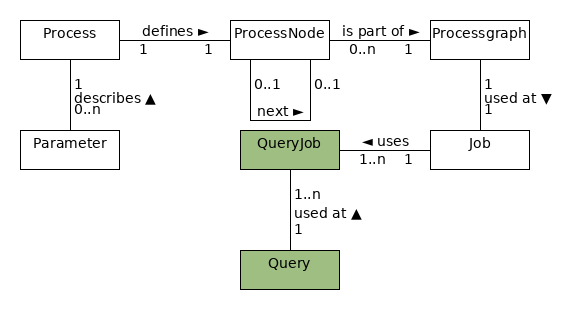
\includegraphics[width=\textwidth]{eodc_eer_rda}
	\caption{Overview of the meta-database of EODC with the proposed additional tables (green).}
	\label{fig:eer_rda} % \label has to be placed AFTER \caption (or \subcaption) to produce correct cross-references.
\end{figure}

\subsection{Query Handler Work-flow}
Figure \ref{fig:impldataid} shows an overview of the data identification solution of the EODC back end. The green parts of the diagram are representing the additions proposed in the thesis. The Query Handler itself is an additional python module in the EODC back end that gets called after the job execution. 

\begin{figure}[h]
	\centering
	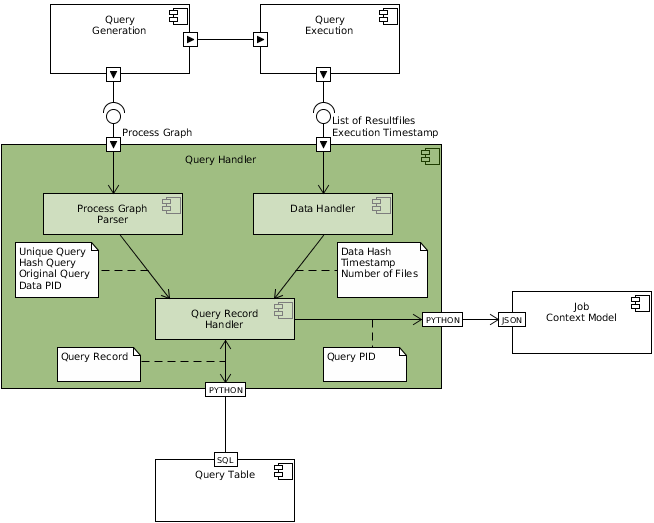
\includegraphics[width=\textwidth]{implementation_dataidentification}
	\caption{Overview of the proposed data identification workflow at the EODC back end}
	\label{fig:impldataid} % \label has to be placed AFTER \caption (or \subcaption) to produce correct cross-references.
\end{figure}


The Query Generation and Query Execution components of the EODC back end provide the input data of the Query Handler. The process graph is the raw input process graph received by the back end driver from the client application. The list of result files is the result of the query execution process and therefore the input data of the work-flow. The Query Execution component provides the execution time stamp additionally. The Query Handler consists of the following components:

 \begin{itemize}
	\item \textbf{Query Processor} \\
	The Query Processor takes the query as input and generates the necessary query data out of it. Since the process graph at this point also includes the processes and not only the filter operations, this step is necessary. The output consists of the original query, the unique/normalized query, the hash of the normalized query and the persisted data identifier of the query. This information is forwarded to the Query Record Handler. The mentioned resulting items are described more in detail in the section below.  
	\item \textbf{Data Handler} \\ 
	The Data Handler is responsible for creating the result data dependent query information. The output is the hash over the file list result, the execution time stamp and additional meta data. In this case the Data Handler only calculates the number of files as meta-data output. Since EODC uses the OGC standard CSW\footnote{http://cite.opengeospatial.org/pub/cite/files/edu/cat/text/main.html} to query the data, the sorting of the resulting files is predefined. The order of the files has no impact on the processing and openEO users are not able to choose a specific sorting, therefore the predefined CSW sorting is used for the hash production. The results of the component is forwarded to the Query Record Handler.    
	\item \textbf{Query Record Handler} \\
	The Query Record Handler communicates with the meta database from EODC to see if an identical Query already exists. The Work-flow of the Query Record Handler can be viewed in Figure \ref{fig:queryhandler_activity}. If the Query Record already exists the Query Record Handler forwards the existing Query PID to the context model, otherwise a new Query PID gets created and persisted in the Query Table. The combination of the result-file hash and the normalized query hash must not have duplicates in the Query table. On saving the Query PID in the job context model, a QueryJob table entry gets created to store the relation between the job id and the Query PID. 
	
\end{itemize}

\begin{figure}[h]
	\centering
	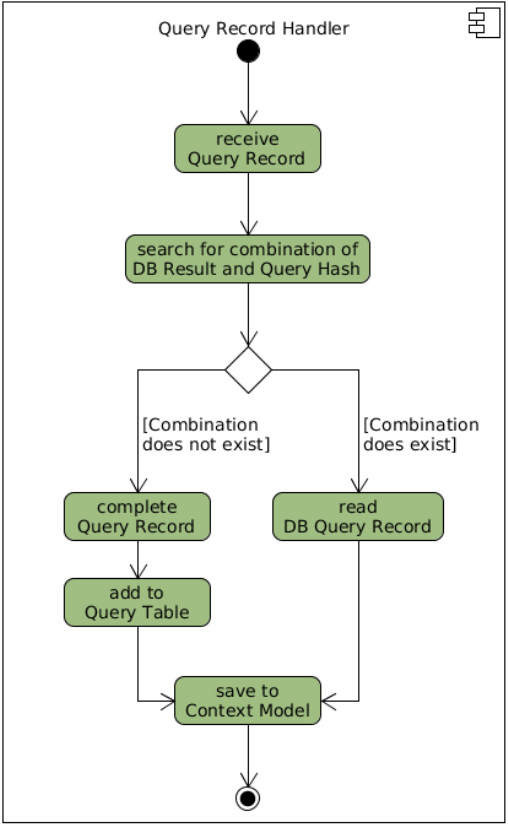
\includegraphics[scale=0.5]{queryhandler_activity}
	\caption{Activity diagram of the Query Record Handler component.}
	\label{fig:queryhandler_activity} % \label has to be placed AFTER \caption (or \subcaption) to produce correct cross-references.
\end{figure}

\subsection{Query Table Structure}

The Query Table stores the data related to the query instance, additional result and meta-data information. Table \ref{Tab:querytable} visualizes the Query Table structure. To illustrate the Query data record, example input values are used to explain how the single data entries are generated. Therefore, in Figure \ref{fig:processgraph_example} there is an example input process graph.   

\begin{figure}[h]
	\centering
	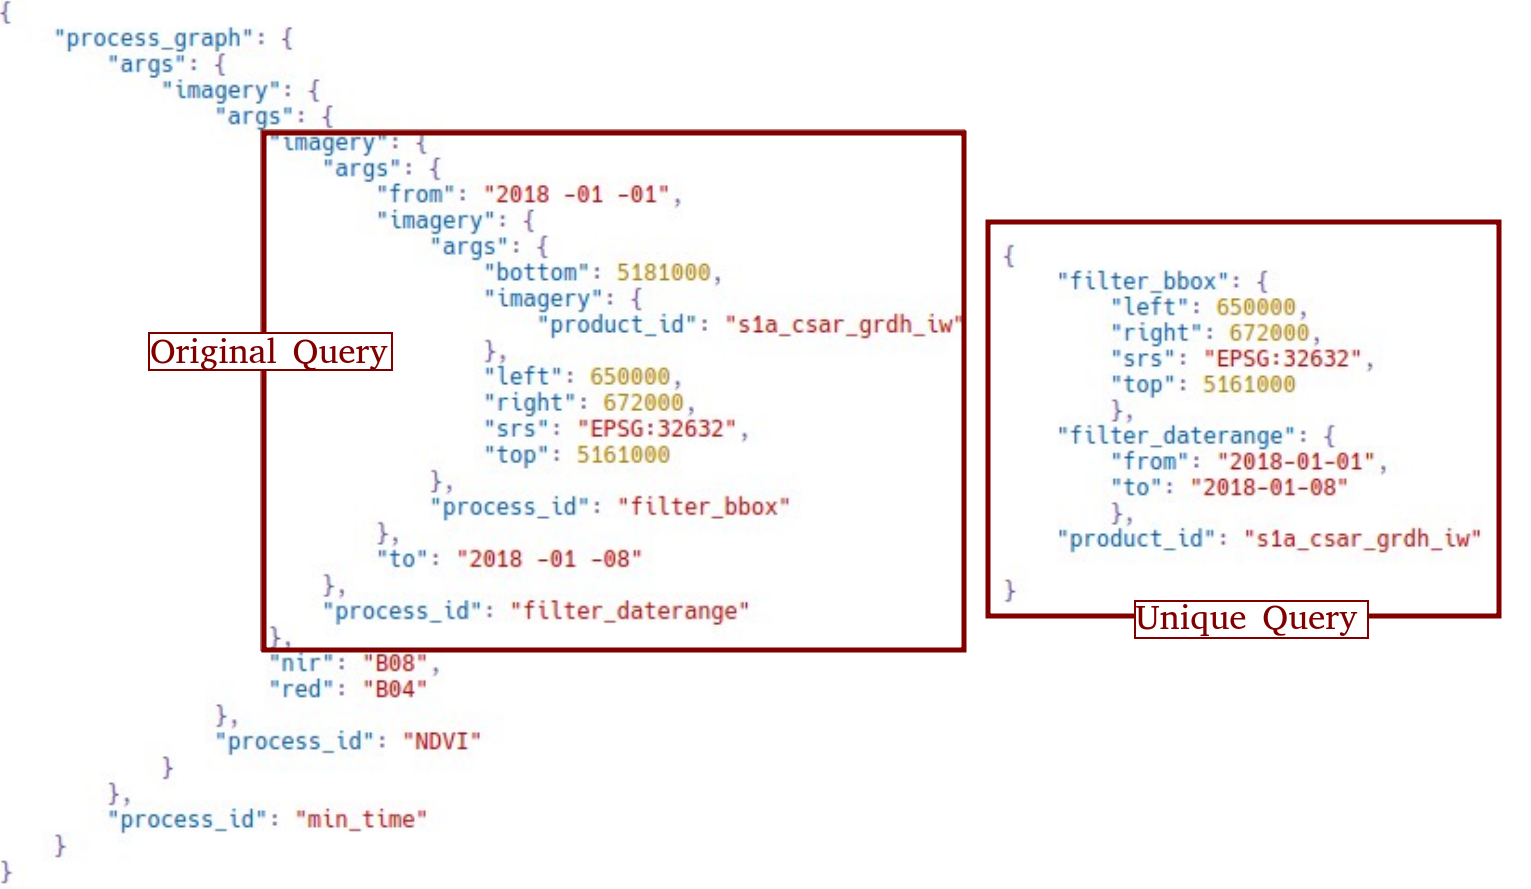
\includegraphics[width=\textwidth]{dataid_example_processgraph}
	\caption{Example Input process graph of the Query Handler component.}
	\label{fig:processgraph_example} % \label has to be placed AFTER \caption (or \subcaption) to produce correct cross-references.
\end{figure} 
\todo{adapt original Query}

\begin{table}[]
	\caption{Structure of the Query Table in the EODC meta database.}
	\begin{tabular}{|l|l|l|l|l|l|l|l|}
	\hline	\textbf{Query} & \textbf{Dataset} & \textbf{Original} & \textbf{Unique} & \textbf{Hash} & \textbf{Hash} &
		\textbf{Exec.} & \textbf{Add.}  \\ 
		\textbf{PID} & \textbf{PID} & \textbf{Query} & \textbf{Query} & \textbf{Query} & \textbf{Result} &
		\textbf{Timest.} & \textbf{Metad.}  \\ \hline
		\textbf{1} & \textbf{2} & \textbf{3} & \textbf{4} & \textbf{5} & \textbf{6} &
		\textbf{7} & \textbf{8} \\ \hline
		\textbf{...} & \textbf{...} & \textbf{...} & \textbf{...} & \textbf{...} & \textbf{...} & \textbf{...} & \textbf{...} \\ \hline
	\end{tabular}
	\label{Tab:querytable}
\end{table}

The following list describes how the elements of the query data set record are created in more detail:

\begin{enumerate}
	\item \textbf{Query PID} \\
	The Query PID gets generated by the python library uuid\footnote{https://docs.python.org/3/library/uuid.html}. The library is used to generate unique identifiers and used in the EODC back end for generating the job ids. In the EODC back end ids have in the beginning a code for the specific entity (e.g. "jb-UUID" for Job entities). That is why the id for a Query Table entry is structured like "qu-UUID". \\
	\textit{Example: "qu-16fd2706-8baf-433b-82eb-8c7fada847da"}
	\item \textbf{Dataset PID} \\
	The dataset PID is the identifier of the satellite in the process graph (e.g. the "product\_id" element). \\
	\textit{Example: "s1a\_csar\_grdh\_iw"}	    	
	\item\textbf{Original Query} \\
	The original query is the input query of from the query execution component, which got executed by it.  \\ 
	\textit{Example: See the Original Query in Figure \ref{fig:processgraph_example}}	 
	\item \textbf{Unique Query} \\
	The unique query is the restructured query that is comparable to other unique queries. Since the order of the filters makes no difference in the outcome of the query execution, the elements of the original query are alphabetically sorted by the JSON keys to get the unique query. \\
	\textit{Example: See the Unique Query in Figure \ref{fig:processgraph_example}}	  	 	
	\item \textbf{Unique Query Hash} \\ 
	Newline and space characters are removed from the unique query string. The unique query hash is the output of the SHA-256 hash function (using the python module "hashlib") with the unique query as input.  \\
	\textit{Example: "AE7EF888CDEDF8A9A371\dots"} 
	\item \textbf{Result Hash} \\
	The result hash is the output of the SHA-256 hash function (using the python module "hashlib") with the result file list as input. Before the list is applied to the hash function it is transformed to a string and the newline and white space characters are removed. \\
	\textit{Example: "565D229FCE4772869343\dots"} 
	\item \textbf{Execution Time-stamp} \\
	The execution time stamp is the input parameter of the Query Handler and is transformed to the data type needed by the data base. The time-stamp is taken by the query execution handler and is part of the query execution result. To forward it to the Query Handler it has to be read from the result object. \\
	\textit{Example: "2018-10-17 18:03:20,609"}  
	\item \textbf{Additional Meta-data} \\
	The additional meta-data column of the Query table can be used by the EODC back end to store additional information about the query execution. In the implementation of this thesis, only the number of output files are persisted in the database. The column is defined as a JSON object and can be extended with additional meta-data easily. \\
	\textit{Example: "\{ "number\_of\_files": 10\}"}    	 
\end{enumerate}

\section{Back end provenance}\label{Implementation:Back end provenance}

The aim of the back end provenance is to persist the versions of the back end and therefore the version of the software used to execute the jobs. The following subsections explain how the, in Section \ref{Design:Back end provenance} defined, provenance data elements are read from the GitHub repository.  

\textbf{B1: GitHub Repository} \\
The GitHub repository is directly used to create the services of the EODC back end. Therefore, the currently used GitHub repository information can be read via the command line interface (CLI) of Git. The used commit and branch are accessed directly via the Git CLI. In the listing below the Git CLI calls used to get the GitHub repository information.       

\begin{lstlisting}[frame=single, language=Python]
# Receiving the Git Repository URL
git config --get remote.origin.url 
# Receiving Branch
git branch
# Receiving the commit messages with the timestamps
git log 
\end{lstlisting}

\textbf{B2: Core API Version} \\
Back end developers manually update the OpenEO core API version of the EODC back end. It is in the GitHub repository of the EODC back end. 

\textbf{B3: Back End Version} \\
Since EODC takes the code for the services directly from GitHub, the Git commit identifier is used as the version of the back end.

\textbf{B4: Publication Time-stamp} \\
The publication time-stamp of the EODC back end is defined by the time-stamp when the Git commit happened. It is persisted by GitHub and can be retrieved via the Git CLI. 
\todo{Maybe add the code example}

\section{Job dependent provenance}\label{Implementation:Job dependent provenance}
The EODC back end of the release version "0.3.1" transforms the process graph into separate docker containers. For every process in the process graph there is a docker container running the related python code. The input of the current process is the output of the previous process. The first process docker container has the input data defined in the process graph as input value, which is the result of the query execution. Every process saves the results in a temporary folder dedicated to the specific process execution. Every process has its own temporary output directory until the whole process chain is finished. After that the back end deletes the temporary folders and only the end result is persisted in the job directory.
To achieve the job environment data capturing described in Chapter \ref{Design:Job dependent provenance}, the processes must provide meta-data about the input data, the output data and the processing itself. \\ 
This thesis describes two different implementations to achieve the job dependent environment capturing. The first implementation uses the python wrapper noWorkflow \cite{c9e0604becba42af96a9cb0a6f60018b}. Instead of calling the processing code with the python interpreter, the noWorkflow wrapper gets called. It automatically creates a meta-data database regarding the python execution. Since the wrapper is capturing the environment in a detailed way, which influences the performance, a second, simpler approach is implemented. Section \ref{Evaluation:NvsP} compares the noWorkflow approach and the second python approach and shows the reasons for using the second approach in detail. The second implementation adds the specific information of interest to the logging of the processing and reads the logging files to generate the context model. This solution modifies and extends the existing python code and is used for the evaluation of this thesis. In Figure \ref{fig:impljobcapture} an overview of the job capturing work-flow is presented. Section \ref{Implementation:Python Implementation} describes the single parts of the overview in more detail.  


\subsection{Context Model Repository}\label{Implementation:Provenance Repository}
Each executed job creates a context model. If the job gets re-executed, the context model gets replaced by the new context model. Job re-execution is internally handled as a new job with the same process graph. The functionality of letting the same job be re-executed without creating a new job id is dropped from the agenda of the OpenEO project in version 0.3.1 (see the GitHub repository\footnote{https://open-eo.github.io/openeo-api/v/0.3.1/apireference/}). 
The context model is stored as a JSON object in the job execution meta-database. After the job is carried out in the EODC back end the results are saved in a folder named after the unique job identifier and the meta data information is stored in a PostGreSQL database (see Section \ref{EODC Back End}). Jobs are saved in the Job table of the database and in this solution the context model is an additional column of it. The context model JSON object gets created by the implementations described below. \\
Table \ref{Tab:contextmodel} provides the mapping between the context model elements from Section \ref{Design} and the keys of the JSON context model object of the prototype. The elements have a one to one mapping of the context model and the JSON key except for the timestamps of the execution. The execution time stamps are part of the Job table in the EODC meta-database. \\
Figure \ref{fig:job_context_model} shows an example context model. It consists of all elements described for the context model in the Design section. Information on the back end environment during the execution of the job is persisted in the context model. In the context model the back end version and the execution time-stamp is persisted and can be used to identify the back end provenance of the execution time. The code environment is a list of all python dependencies with their versions installed during the execution of the jobs. In addition the python interpreter version is added to the JSON object. How the data is captured in detail is described in the sections below.    

\todo{Make Glossary !}
\todo{Add listing captions !}
 
\begin{table}[]
	\caption{Relation of context model elements and EODC JSON context model.}
	\begin{tabular}{l|l}
		\textbf{Context Model Definition} & \textbf{JSON Key} \\ \hline
		\textbf{J1: Input data persistent identifier} & input\_data \\ \hline
		\textbf{J2: Back end provenance / code identifier} & backend\_env \\ \hline
		\textbf{J3: Programming language} & interpreter \\ \hline
		\textbf{J4: Installed packages of the programming language} & code\_env \\ \hline
		\textbf{J5: Start and end time of the process execution} & start\_time, end\_time \\ \hline
		\textbf{J6: Result hash} & output\_data \\ %\hline
	%	\textbf{J7: Back end provenance} & backend\_env \\ 
	\end{tabular}
\label{Tab:contextmodel}
\end{table}

\begin{figure}[h]
	\centering
	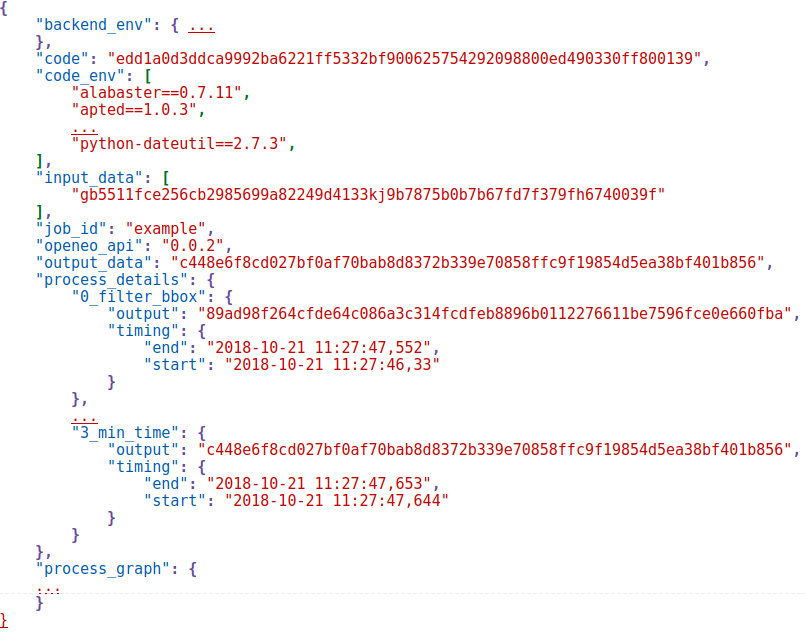
\includegraphics[width=\textwidth]{job_context_model}
	\caption{Example context model of a job execution at the EODC back end.}
	\label{fig:job_context_model} % \label has to be placed AFTER \caption (or \subcaption) to produce correct cross-references.
\end{figure}

\subsection{Python Implementation}\label{Implementation:Python Implementation}
The EODC implementation proposed by this thesis is an example for other back ends, hence needs to be easy to implement and maintain. Therefore, the implementation is done in the python version of the EODC back end without any additional requirements. The python solution uses logging messages to transfer the needed data from the process execution program to the capturing tool. The cleanup service of the EODC back end driver triggers the execution of it. It is an additional python module and parses the log files after the job is finished. This solution generates, except for the additional logging calls, little impact on the existing back end implementation. The EODC back end driver has already a logging system installed, hence the modifications are added in the existing logging policy. \\
Figure \ref{fig:impljobcapture} visualizes the additional python module \textit{Job Capturing} and \textit{Result Handler} in the context of the back end environment. The following list describes the work-flow of the solution at the EODC back end driver. 

\begin{figure}[h]
	\centering
	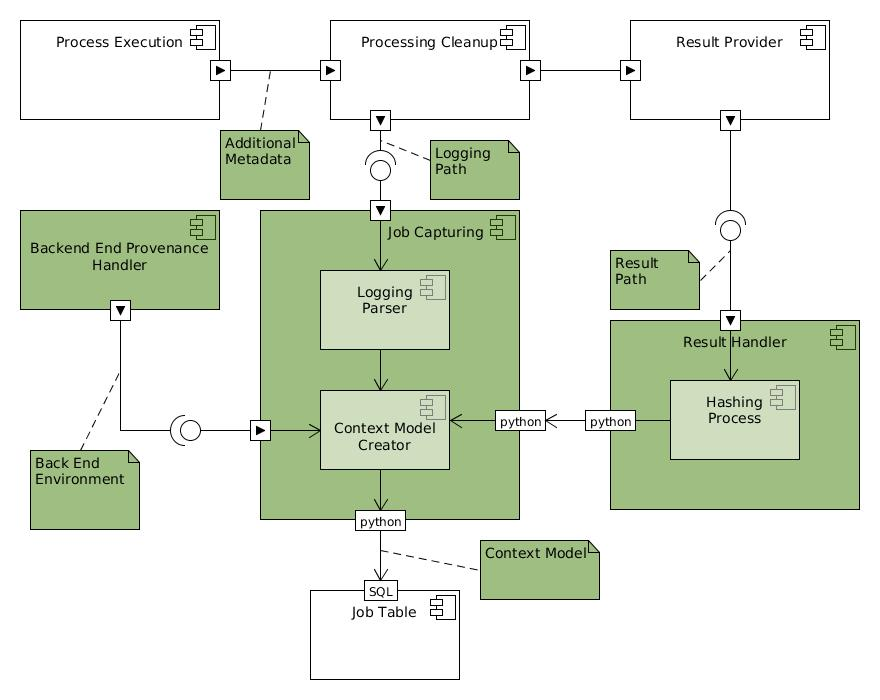
\includegraphics[width=\textwidth]{job_capturing_overview}
	\caption{Overview of the Job capturing architecture at the EODC back end}
	\label{fig:impljobcapture} % \label has to be placed AFTER \caption (or \subcaption) to produce correct cross-references.
\end{figure}

\begin{enumerate}
	\item \textbf{Process Execution} \\
	The \textit{Process Execution} module at the EODC back end is responsible for the actual execution of the job. It creates the additional logging information (J1, J3, J4 and J5) and persists it in the logging file of the job execution. 
	\item \textbf{Processing Cleanup} \\
	After the job execution is finished, the temporary folders are deleted from the file system and the result is copied to the persisted job folder. Then the additional \textit{Job Capturing} module starts with the path to the logging file.  
	\item \textbf{Result Provider} \\
	The \textit{Result Provider} is responsible of making the result available for the user and providing the user with the feedback of the finished job. In addition it invokes the added \textit{Result Handler} module with the path of the resulting file.
	\item \textbf{Result Handler} \\
	The \textit{Result Handler} reads the result file and calculates an SHA-256 hash over it. After completion it is provided to the \textit{Context Model Creator} module.  
	\item \textbf{Job Capturing} \\
	The \textit{Job Capturing} module parses the logging file to extract the information needed for the context model (J1, J3, J4 and J5) and passes the formatted information to the \textit{Context Model Creator}. The \textit{Context Model Creator} needs the \textit{Result Handler} (J6) and \textit{Back End Provenance Handler} (J2) for the remaining parts of the context model. After receiving all necessary information the JSON context model is created and stored to the Job table in the EODC meta-database.    
\end{enumerate}

The following sections describe the capturing of each data element of the job dependent context model in more detail.

\textbf{J1:  Source Input Data Identifier} \\
The source input data identifier is the pid of the input data and query provided by the EODC query store described in Section \ref{Implementation:Data Identification}. It is forwarded to the \textit{Job Capturing} module by the \textit{Processing Cleanup} module. 

\textbf{J2: Back end provenance / Code Identifier} \\
The \textit{Job Capturing} module reads the back end provenance from the \textit{BackendMonit} output JSON file described in Section \ref{Implementation:Back end provenance}. The latest back end version during the execution is copied to the context model.

\textbf{J3 and J4: Programming language and  installed packages of programming language} \\
The \textit{Process Execution} module uses the installed python module \textit{pip} to list all installed packages including their versions. The module is at the moment used to manage the python packages of the back end. The GitHub repository of the EODC back end driver includes a python environment file to automatically install all needed dependencies of python via \textit{pip}. A feature of that tool is the \textit{pip freeze} call, which returns all installed python packages including their concrete versions. This is then transformed to a JSON list object and saved to the context model. In addition to this the \textit{Process Execution} captures the python version by using the \textit{sys.version} call. All of this executions are done in the \textit{Process Execution} module, in the actual processing environment and stored in the output log file of the job execution.    

\textbf{J5: Start and end time of process execution} \\
The start and end time of the process execution is already done at the EODC back end in the  \textit{Process Execution} module. The resulting time stamps are persisted in the Job table of the meta-database. The \textit{Process Execution} module adds the values to the output logging file. These logging entries are not added by this solution, since they are already implemented by the EODC back end provider.  

\textbf{J6: Result Identifier } \\
The result identifier consists of the resulting data of the whole process graph execution. It is a SHA-256 hash (using the \textit{hashlib} python library) of the resulting alphabetical sorted output files, which are placed in the resulting folder of the job execution directory. In the current version of the back end there is only one result file created, due to the limitations of the available processes.  


\subsection{Alternative Implementation}\label{Implementation:Noworkflow Implementation}
NoWorkflow is a python module used to capture the provenance of a python script execution. The main aim of it is that the program itself does not have to be changed, it only has to be executed with the noWorkflow interpreter instead of python. It then automatically creates a provenance database on every execution of the script called “trial”. Every time the job gets executed a new trial is created. A trial in the past can be re-executed with the same conditions and trials themselves can be easily compared and visualized with noWorkflow (see \cite{c9e0604becba42af96a9cb0a6f60018b}). NoWorkflow and its capabilities are described in Section \ref{Noworkflow}. 
For the purpose of the job dependent provenance capturing described in the Design section, only parts of the provenance capturing functionality that noWorkflow offers is suitable. In the following the features of noWorkflow used in the alternative implementation that differ from the actual solution at Section \ref{Implementation:Python Implementation} are presented.    


\textbf{J2: Back end provenance / Code Identifier} \\
The job identifier is defined by the back end version, which includes the current state of the locally checked out GitHub repository.\\
To enable a more detailed environment, noWorkflow captures the hash of the executed code. The hash from the database of noWorkflow gets retrieved via the command line interface. It contains the command “show” (see code block below), which returns the data of a specific trial. The code hash is extracted from the output and added to the context model. 

\begin{lstlisting}[frame=single]
now show --dir=JOB_DIR
\end{lstlisting}

\textbf{J3 and J4: Programming language and  installed packages of programming language} \\
NoWorkflow captures the used python packages in the database. To retrieve the modules the command line interface is used with the “-m” argument (see code block below), which returns all used python modules including their versions and the version of python. The advantage of using noWorkflow instead of the \textit{pip} tool described in the python solution is that only the used packages are listed.

\begin{lstlisting}[frame=single]
now show -m --dir=JOB_DIR
\end{lstlisting}

\section{User Services}\label{Implementation:User Interface}
The previous sections describe only the technical insight of the back end. This section describes the implementation of the interfaces for the users. Therefore, endpoints are added to the current existing OpenEO core API version 0.3.1. In addition, the proposed endpoints are applied to the python client and the EODC back end. The implementation of the recommended additions of Section \ref{Design:User Interface} are described in the following:

\textbf{Implementation of U1: Back end version} \\
Retrieving additional information about the back end was added into a new end point of the API. The new endpoint is a GET request called “/version” and no authentication is needed to access it. Response of the version endpoint is the whole job independent provenance information of the back end (B1-B5, see Section \ref{Implementation:Back end provenance}). In a production version, the data may be filtered for information marked as a security risk. This endpoint is added to the EODC back end to return the latest back end version including meta-data. The endpoint takes a time-stamp as parameter to get the back end version meta-data of a specific time. Further additions are created to the python client, so that the user can call a method in the python client called “version()” to retrieve the information of the back end directly in the python client. The result is a JSON object consisting of the back end provenance data \todo{like in Figure \ref{fig:backendprovcm}. change to picture in the use cases section}

\textbf{Implementation of U2: Detailed Job Information} \\
In the OpenEO coreAPI there is an endpoint to get detailed information about the job status. The endpoint path is “GET /jobs/<job\_id>” , which by the current release version of 0.3.1 only contains the execution state of the job and the job id. In addition to this the available information of the whole job dependent provenance gets added to this endpoint in the implementation of this thesis (e.g. see Figure \ref{fig:job_context_model}). Since the python client just returns the resulting JSON response from the back end as a python dictionary, there is no modification needed.

\textbf{Implementation of U3: Comparing two Jobs} \\
The core API does not define the comparison of two jobs, hence there does not exist any user interface. The modified core API defines a new endpoint in the manner of existing endpoint definitions. For the purpose of this thesis the endpoint  “POST /jobs/<job\_id>/diff” gets introduced to the new core API. In the url of the request the user defines the base job id, which context model will be compared with other jobs. In the body of the request the target job ids are defined in a JSON list. After getting the request from the user, the back end compares the context models of the base job with every target job occurring in the request body list. The result from the back end consists of, for every item in the base job context model, the term “EQUAL”, if the item is the same in both context models, the difference if the items are not the same in both context models, or “MISSING” if the item is in the base job context model, but missing in the target job context model or the other way around. If an element is different, the elements that differ are visible. The latest mentioned outcome can occur if the context model definition is modified in future job executions and there are e.g. additional fields of it. The response contains the context model of all jobs with one of the previously described three states inside of every items value. In the python client this feature is added with an additional function of the Job class called "diff(target\_job)". Figure \ref{fig:job_comparison} provides an example of the dictionary output of this function.
\todo{Change figure to one in the Use Cases section}
\begin{figure}[h]
	\centering
	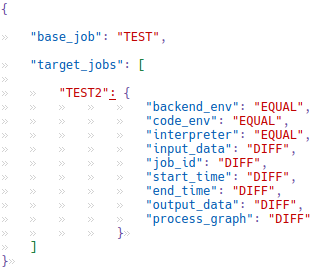
\includegraphics[scale=1]{job_comparison}
	\caption{JSON Example of a job comparison result.}
	\label{fig:job_comparison} % \label has to be placed AFTER \caption (or \subcaption) to produce correct cross-references.
\end{figure}



\textbf{U4: Data Identifier Landing Page} \\
Depending on the back end, the input data may be restricted to the OpenEO interface. Therefore, the resolver of the input data PID is set within the core-API specification. In the coreAPI release version 0.3.1, there exists an endpoint to retrieve detailed information about a data set. The "GET /collections/<dataset-id>" endpoint is extended, by accepting query PIDs. If the user calls the endpoint with a data PID, the result are the details of the underlying dataset and in addition the result of the query execution and the original query parameters. The landing page contains a link to another page with the file list after a query re-execution ("GET /collections/<data-pid>/result" endpoint). If the result file list differs from the original execution, there will be a warning message added to the response. 

\textbf{U5: Re-use of Input Data} \\
To re-use the input data in a different job execution, the data PID can be used in the process graph directly as source data, instead of just the unfiltered dataset identifier. If a process graph uses the input data PID, the EODC back end automatically applies the queries in a way of the original execution. To pass the data PID to the process graph, it is inserted in the "product\_id" entry. Section \ref{Implementation:Use Case1} provides an example of such a process graph. If the query result data changed from the original execution of the PID, the job shall be processed anyway, but there has to be a warning message to notify the user.  

\section{Use Cases}
This section shows how the use cases of Section \ref{Use Cases} can be addressed using the implementation described in the sections before.

\subsection{Re-Use of Input Data}\label{Implementation:Use Case1}
The first scenario describes the process of a researcher using OpenEO as processing environment. In this use case the focus is on the data identification and data citation part of the solution. Researchers that use OpenEO may want to cite the data that is used in the applied process chain. Other scientist then may want to use this data in their related research experiment. The step-by-step description of the scenario can be viewed in the Section \ref{UseCase1}. In this section the steps of the use case are executed at the evaluation environment.
\todo{add Footnote / Link to GitHub Repo}
\begin{enumerate}
	\item \textbf{Researcher A runs an experiment (job A) at the EODC back end.} \\
	This step is basic OpenEO functionality and is not influenced by the solution from the user point of view. The researcher chooses Sentinel-2 data by loading the Sentinel-2 collection of EODC with the data-set identifier "s2a\_prd\_msil1c". In the next step the data is filtered temporally (May of 2017) and spatially (bounding box of the south tyrol area). In the next step the researcher applies the NDVI\footnote{https://earthobservatory.nasa.gov/features/MeasuringVegetation/measuring\_vegetation\_2.php} process on the filtered data as well as the minimum value of each pixel in the time range with the "min\_time" process. The NDVI calculation needs the measurements of the satellite in near-infrared (parameter "nir") and the measurements of red light (parameter "red"). for Sentinel 2 data of the EODC the two measurements are represented by the band identifiers "B08" for near-infrared and "B04" for visible red light. The last two lines create a job at the back end with the specified process graph and start the execution of it.
	At the back end the Query Handler is generating a new data PID or returns an already existing one if the same query got executed in the past. The following python client code represents the experiment of Researcher A.  
	\begin{lstlisting}[caption={Researcher A runs job A with the python client}, captionpos=b,frame=single, language=Python,label={lst:impl_usecase1_1}]
import openeo
EODC_DRIVER_URL = "http://openeo.local.127.0.0.1.nip.io"
		
con = openeo.connect(EODC_DRIVER_URL)
	
# Choose dataset
processes = con.get_processes()
pgA = processes.get_collection(name="s2a_prd_msil1c")
pgA = processes.filter_daterange(pgA, extent=["2017-05-01", 
                                              "2017-05-31"])
pgA = processes.filter_bbox(pgA, west=10.288696, 
		south=45.935871, east=12.189331, 
		north=46.905246, crs="EPSG:4326")
	
# Choose processes
pgA = processes.ndvi(pgA, nir="B08", red="B04")
pgA = processes.min_time(pgA)
	
# Create job A out of the process graph A (pgA)
	
jobA = con.create_job(pgA.graph)
jobA.start_job()
	\end{lstlisting}
	
\todo{Add result of use case 1 image}

	\item \textbf{Researcher A retrieves the used input data of job A.} \\
	If Researcher A wants to receive the input data identifier, the job description endpoint has to be called. The following code snipped shows the call using the python client.
	
	\begin{lstlisting}[caption={Researcher A retrieves the used input data pid}, captionpos=b,frame=single, language=Python,label={lst:impl_usecase1_2}]
pidA_url = jobA.get_data_pid_url()
print(pidA_url)
# Output: EODC_DRIVER_URL/collections
#	/qu-d1701f4e-e7c5-4a83-92e0-9facbd401a06
pidA = jobA.get_data_pid()

# retrieve information about the pidA 
# e.g. executed query and description about the dataset.
desc = con.describe_collection(pidA)
	
query = desc["query"]
# re-execute query and get the resulting 
# file list from the back end
file_list = con.get_filelist(pidA)
	\end{lstlisting}
	
	\begin{figure}[h]
		\centering
		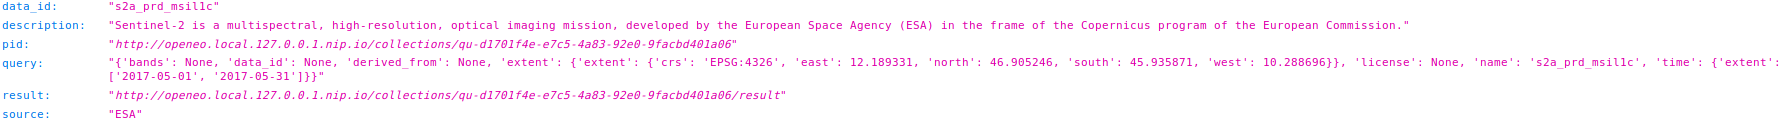
\includegraphics[width=\textwidth]{usecase1_2}
		\caption{Screenshot of the job A landing page.}
		\label{fig:usecase1-pid} % \label has to be placed AFTER \caption (or \subcaption) to produce correct cross-references.
	\end{figure}	
	The job\_details variable is an unfiltered python dictionary object that contains the response of the EODC back end. It has a data element at the key of "input\_data" that consists of the input data PID as a resolvable web address. Figure \ref{fig:usecase1-pid} shows the response data of the query PID information. After calling the page, the user is provided by the executed filter parameter, the dataset identifier, a description about the dataset. In addition the link to get the re-execution results of the query and the resolvable query pid is added to the page (see Figure \ref{fig:usecase1-pid}). \\
	To gather the information about the input data directly in the python client code, the last three calls of the code block above can be used.  
	
	\item \textbf{Researcher A cites the input data in a publication.} \\
	This step is independent from the implementation and therefore not explained in detail. For the further steps it is assumed that Researcher A used the resolvable PID from step 2 (\textit{"EODC\_DRIVER\_URL/collections/qu-d1701f4e-e7c5-4a83-92e0-9facbd401a06"}) for the citation.   
	
	\item \textbf{Researcher B uses the same input data of job A for job B.} \\
	In order to use the same input data as Researcher A, Researcher B uses the data PID from the publication and puts it into the input data element of the process chain of job B. In the block below an example of code needed to use the same input with a different process chain (max\_time instead of min\_time process) is printed.   
	\begin{lstlisting}[caption={Researcher B uses pid A for different job.}, captionpos=b,frame=single, language=Python,label={lst:impl_usecase1_3}]
import openeo
	
# Take input data of job A by using the input data pid A
# pidA = qu-d1701f4e-e7c5-4a83-92e0-9facbd401a06
pgB = processes.get_collection(
      data_pid="qu-d1701f4e-e7c5-4a83-92e0-9facbd401a06")
# Alternative: data_pid="EODC_DRIVER_URL/collections/pidA" 
	
# Choose processes
pgB = processes.ndvi(pgB, nir="B08", red="B04")
pgB = processes.max_time(pgB)
	
# Create job B out of the process graph B (pgB)
	
jobB = con.create_job(pgB.graph)
jobB.start_job()
	\end{lstlisting}
	
\end{enumerate}
\todo{Add result of use case 1 - 4 image}
\subsection{Capturing job dependent environments}\label{Implementation:Use Case2}
This scenario focuses on the execution environment. It handles the need of researchers to describe the execution process. The implementation at the EODC back end gives the users the option to gain additional meta-data about the execution. In the following the steps of the scenario are run with the implemented instance of the EODC back end.    

\begin{enumerate}
	\item \textbf{Researcher runs an experiment (job A) at a back end.}\\
	The researcher A runs a job at the EODC back end with the following python client code. This is the default workflow of executing a job using the python client.  
	\begin{lstlisting}[caption={Researcher A runs job A with the python client}, captionpos=b,frame=single, language=Python,label={lst:impl_usecase2_1}]
import openeo
EODC_DRIVER_URL = "http://openeo.local.127.0.0.1.nip.io"
		
con = openeo.connect(EODC_DRIVER_URL)
	
# Choose dataset
processes = con.get_processes()
pgA = processes.get_collection(name="s2a_prd_msil1c")
pgA = processes.filter_daterange(pgA, extent=["2017-05-01", 
                                              "2017-05-31"])
pgA = processes.filter_bbox(pgA, west=10.288696, 
                south=45.935871, east=12.189331, 
                 north=46.905246, crs="EPSG:4326")
	
# Choose processes
pgA = processes.ndvi(pgA, nir="B08", red="B04")
pgA = processes.min_time(pgA)
	
# Create job A out of the process graph A (pgA)
jobA = con.create_job(pgA.graph)
jobA.start_job()
	\end{lstlisting}
	\item \textbf{Researcher wants to describe the experiment environment.}\\
	The researcher wants to publish the result of the experiment and therefore needs to describe the environment in detail. The following code-lines provide the user with detailed information about the job execution:
	\begin{lstlisting}[caption={Describe jobA execution environment}, captionpos=b,frame=single, language=Python,label={lst:impl_usecase2_2}]
# Get context model of job A
context_model = jobA.describe_job["context_model"]
	
# Retrieve the information that Researcher A needs.
	
interpreter = context_model["interpreter"]
code_env = context_model["code_env"]
input_data = jobA.get_data_pid_url()
backend_version = jobA.get_backend_version()
logging.info("Interpreter: {}".format(interpreter))
logging.info("Code Environment: {}".format(code_env))
logging.info("Input Data PID URL: {}".format(input_data))
logging.info("Back End Version (commit): {}".format(backend_version["commit"]))
	\end{lstlisting}
	After the execution of the lines above, the researcher is able to get the used programming language including the version and installed packages. In addition the back end version describes the used processing code. For more transparency the researcher can link to the used GitHub repository and the commit used for the experiment. Figure \ref{fig:usecase2_2} shows the output of the logging calls. 
	
\end{enumerate}

\begin{figure}[h]
	\centering
	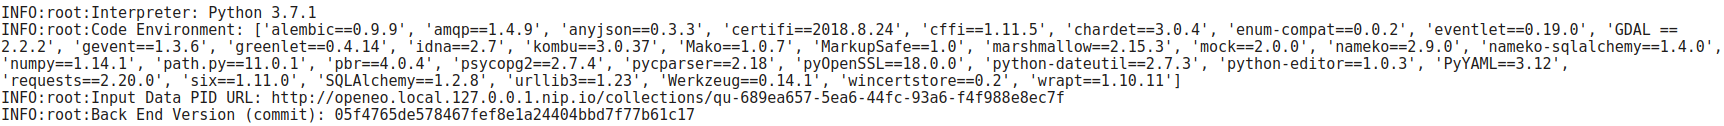
\includegraphics[width=\textwidth]{usecase2_2}
	\caption{Screenshot of logging output of the second Use Case.}
	\label{fig:usecase2_2} % \label has to be placed AFTER \caption (or \subcaption) to produce correct cross-references.
\end{figure}

\subsection{Getting differences of job executions}\label{Implementation:Use Case3}
The last use case is focused on the users of OpenEO. It describes the need of transparency of job executions for the users. If results differ with the same job later in time, the user can access meta-data to find reasons why it happened. Other users might compare different job execution environments.  
\begin{enumerate}
	\item \textbf{Researcher runs an experiment (job A) at a back end.}\\
	The researcher A runs a job at the EODC back end with the following python client code. 
	\begin{lstlisting}[caption={Researcher A runs job A with the python client}, captionpos=b,frame=single, language=Python,label={lst:impl_usecase3_1}]
import openeo
EODC_DRIVER_URL = "http://openeo.local.127.0.0.1.nip.io"

con = openeo.connect(EODC_DRIVER_URL)

# Choose dataset
processes = con.get_processes()
pgA = processes.get_collection(name="s2a_prd_msil1c")
pgA = processes.filter_daterange(pgA, extent=["2017-05-01", 
"2017-05-31"])
pgA = processes.filter_bbox(pgA, west=10.288696, 
south=45.935871, east=12.189331, 
north=46.905246, crs="EPSG:4326")

# Choose processes
pgA = processes.ndvi(pgA, nir="B08", red="B04")
pgA = processes.min_time(pgA)

# Create job A out of the process graph A (pgA)

jobA = con.create_job(pgA.graph)
jobA.start_job()
\end{lstlisting}
	\item \textbf{Researcher re-runs the same experiment (job B).}\\
	Since re-execution of the same job id is handled internally with the re-execution of the same job configuration with a new job id, the the following code is used to create the same job again (job B). It uses the same process graph and the definition of pgA is the same as in Listing \ref{lst:impl_usecase3_1}:
	\begin{lstlisting}[caption={Researcher re-reuns job A resulting in job B.}, captionpos=b,frame=single, language=Python,label={lst:impl_usecase3_2}]
jobA = con.create_job(pgA.graph)
jobA.start_job()
	\end{lstlisting}
	
	\item \textbf{Researcher runs a different experiment (job C).}\\
	The third job (job C) is created with a different process configuration and input data query.
	\begin{lstlisting}[caption={Researcher runs experiment different from job A.}, captionpos=b,frame=single, language=Python,label={lst:impl_usecase3_3}]
# Choose dataset
processes = con.get_processes()
pgC = processes.get_collection(name="s2a_prd_msil1c")
pgC = processes.filter_daterange(pgC, extent=["2017-05-01", "2017-05-31"])
pgC = processes.filter_bbox(pgC, west=10.288696, south=45.935871, east=12.189331, north=46.905246, crs="EPSG:4326")

# Choose processes
pgC = processes.ndvi(pgC, nir="B08", red="B04")
pgC = processes.max_time(pgC) # differs from job A

# Create job C out of the process graph C (pgC)

jobC = con.create_job(pgC.graph)
jobC.start_job()
	\end{lstlisting}   
	\item \textbf{Researcher wants to compare the jobs by their environment and outcome.}\\
	Now the researcher wants to compare job B and job C with the first job A. Therefore the following code has to be executed:
	\begin{lstlisting}[caption={Researcher compares the different jobs.}, captionpos=b,frame=single, language=Python,label={lst:impl_usecase3_4}]
diffAB = jobA.diff(jobB)
diffAC = jobA.diff(jobC)
logging.info(diffAB)
logging.info(diffAC)
	\end{lstlisting}  
	With the lines above the researcher gets two dictionaries of the comparisons between job A with job B (diffAB) and job A with job C (diffAC). The content of the dictionary is a comparison of every key of the jobs context model with each other. Figure \ref{fig:eva_diff} is a screenshot of the logging messages defined in Listing \ref{lst:impl_usecase3_4}.
\end{enumerate}

\begin{figure}[h]
	\centering
	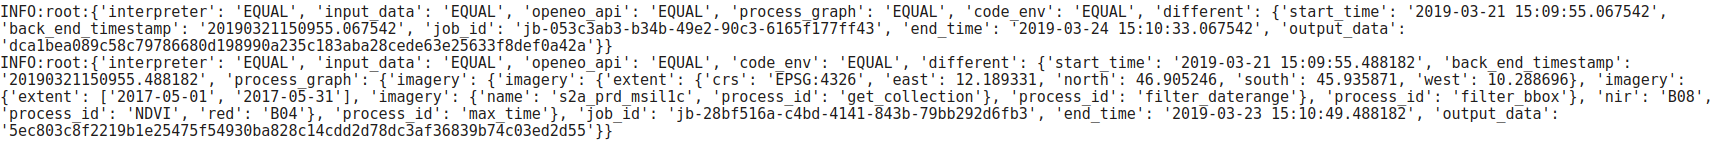
\includegraphics[width=\textwidth]{usecase3_4}
	\caption{Logging output of the job comparisons diffAB and diffAC.}
	\label{fig:eva_diff} % \label has to be placed AFTER \caption (or \subcaption) to produce correct cross-references.
\end{figure}
\todo{store results somewhere}
\section{Summary}
This chapter presented an implementation of the design of Chapter \ref{Design} at the EODC back end. It consists of an implementation of the RDA recommendations for the back end. The additional modules needed to achieve this are presented in Section \ref{Implementation:Data Identification} and are using the CSW\footnote{http://cite.opengeospatial.org/pub/cite/files/edu/cat/text/main.html} Query system. The implementation of the back end provenance uses the advantages of GitHub on versioning the used software and persisting the software versions of the past. The job dependent environment is captured by retrieving the python environment using pip and capturing the version of the software at the execution time. The logging system of the EODC back end is used to communicate the meta-data needed by the context model without changing the processing code. The data of the query and the context model are persisted in additions to the existing PostgreSQL database. In addition the endpoints needed to access the provenance information are inserted into the OpenEO API. In the last section of the chapter, the implementation of the defined Use Cases of Section \ref{Use Cases} are presented. The next chapter evaluates the implementation by the impact on the EODC back end and by testing the implementation against special cases.    

\chapter{Evaluation}\label{Evaluation}
This chapter evaluates the prototype implementation described in the previous section. The work-flow of the evaluation is applying the three use cases defined in Section \ref{Use Cases} to the solution of Section \ref{Implementation:Python Implementation} and evaluate if the outcome reaches the expectations.\\ First the set up of the evaluation environment is described in Section \ref{Evaluation:Setup}. \\ Section \ref{Evaluation:special} evaluates how the solution behaves on special circumstances. \\ Section \ref{Evaluation:impact} evaluates the impact of the solution to the EODC back end by looking into storage and performance metrics. \\ The last section in this chapter presents a comparison between the used python implementation and the noWorkflow implementation described in Section \ref{Implementation:Noworkflow Implementation} on different aspects. Since the amount of resulting information can be very big, only the important information is extracted from the communication in the next sections.


\section{Evaluation Setup}\label{Evaluation:Setup}
The EODC back end provides the evaluation setup for testing the prototype of this thesis. It is a duplicate of the productive service running at the OpenEO back end. EODC uses the Open Shift service to provide the back ends functionality. It uses the version provided at GitHub from EODC to build the local instance of the EODC back end. In this setup a GitHub fork of the EODC back end is used to deploy the adapted back end of Section \ref{Implementation}. Since the used back end instance is a duplicate of the actual productive service, the data used in the back end is the actual data that EODC provides for the OpenEO users. Changes on the data (like removed files or updated files) are simulated by changing the output of the query directly after execution. This allows for an unrestricted evaluation of the use cases. If the changes suit EODC, it can switch easily the productive instance with this test instance. \\
The evaluation is done from a user point of view, hence an OpenEO client needs to be used for the evaluation. The python client is chosen for this purpose including the additional functionality described in Section \ref{Implementation:User Interface}. \\ 
\todo{Extend this by the laptop settings}
\section{Special Test Cases}\label{Evaluation:special}
This section evaluates special test cases to get an overview on how the solution behaves, if specific circumstances occur. These test cases are created to look into the error proneness of the solution. They are structured by the topic of the test cases in the following sections.

\subsection{Data Changes}\label{Evaluation:special_dataid}
This section describes situations, where data changes on the EODC back end occur. The data of EODC can not be changed, since the evaluation back end is using the actual data. To simulate changes on the data, the query result received by the back end driver gets modified. What data will be modified is described by the test cases below. The policy of the EODC back end regarding updates on data sets is to create a new filename for the updated data record. The filename is the identifier of the data set and will never stay the same, if the content of it gets changed. The new filename is then inside of the query result instead of the original filename. Usually if this happens at the EODC back end, the original data record gets deleted. Hence, updates on the data can be simulated by renaming the input files. The running job (referenced as JobA) defined in Section \ref{example} is used for this purpose. \\
The following steps are taken to test the behavior on data changes:
\todo{Update text with local CSW server}
\todo{Show concrete code of execution}
\begin{enumerate}
	\item \textbf{Run JobA, which creates query PID-A. Get file list of PID-A} \\
	After executing the job the PID-A is created as "qu-4dc4e155-cd36-4f90-a335-f610b58fec7a". The resulting file list consists of 31 files. One of the filenames ends with "T32TPR\_20170104T101405.zip". 
	\item \textbf{Change filename of one File of PID-A query resulting files} \\
	The file with the name ending with "T32TPR\_20170104T101405.zip" is now set to end with "T32TPR\_20170104T101405\_NEW.zip", by replacing the name after the query execution. Since the processing would break, if the name is changed in that way, it is replaced by the original name for the processing service.  
	\item \textbf{Get file list of PID-A} \\
	The second call for the file list, after the file is modified results in a different file list and a warning message, that the resulting files differ from the original execution.
	\todo{describe how it works with the timestamp}
	\item \textbf{Run duplicate of JobA} \\
	After running a duplicate of JobA, a new query PID ("qu-5ad7c999-058b-4560-a1fc-25195a448c65") gets created, which is correct behavior since the result of the query changed. 
	\item \textbf{Run JobB using PID-A}\\
	JobB is the same process chain as JobA, but using the data PID of JobA as input parameter. After executing JobB, the job gets the same input data PID as the duplicate of JobA ("qu-5ad7c999-058b-4560-a1fc-25195a448c65") instead of the used PID-A. The job got executed by the updated data records, since the execution of the same query returns a different resulting data. In the job description endpoint there is a warning message, that the data input was different to the specified input data PID of the process graph. 
\end{enumerate}
\todo{Show select * from the database}
\todo{Show how it works with the timestamps}
The test case shows the behavior of the solution, if the data gets updated, nevertheless the behavior is the same for deleted data records. The deletion changes the outcome of the query execution and therefore, a new query PID gets generated. Another outcome of the example is that the used input data PID of a job execution is consistent only after the execution. It shows limitations of the EODC back end at the moment for not being able to query for deprecated data records. Nevertheless, the implementation gives the user the possibility to notice changes in the data-set. \\
The remaining question is how the system behaves if the data is updated during the query processing. Since there is no permission to perform a test on it, it can only be assumed theoretically. Since the query system is file based and an update results in a new file replacing an existing file. There are two possibilities of the outcome of a query be executed at the same time. Either the query results in the old file, which then will result in an error at the execution if the file is replaced already at the time of the job execution, or the query results in the new file. In both cases the query PID will be generated consistent with the job execution, since it takes the original executed query and the actual file list used for the execution.     

\subsection{Job Capturing}\label{Evaluation:special_jobcap}

This section reviews the outcome of the job capturing critically. The focus of it is the created context model of the job executions. The following two question are used to discuss the impact of the captured data regarding the job execution.  \\

\textbf{Is it theoretically possible to recreate an older version of the back end?} \\
The aim of the implementation is to capture enough data to make it theoretically possible to re-run the same job. The EODC back end is created directly by a GitHub repository. To recreate an old version of the back end, the GitHub repository URL and the commit identifier of the original set up is needed. The timestamp of the job execution is persisted in the context model of the original job execution. The original GitHub repository and commit can be resolved by the back end provenance. Therefore, the information of re-creating the back end state from an older version is captured. To re-create the original job on the back end, the process graph of it is persisted and can be re-executed. The execution of the job is the same, assuming the input data has not been deleted in the meantime. The result hash makes it possible to validate, if the job re-execution was the same.

\section{Impact}\label{Evaluation:impact}

This section evaluates the impact of the implementation on the EODC back end. To achieve this a testing set of 25 different process graphs are executed at the EODC back end. The testing set consists of a composition of jobs with different complexity. There are 15 jobs in the same complexity level of the running example (estimated 2MegaBytes (MB) result file), where every job creates a new input data PID. There are 5 jobs that are using existing input data PIDs and 5 jobs with a big area of interest, which will lead to a resulting output file of about 25MB. The impact is measured by the impact on the performance and the impact on the storage of the EODC back end.           

\subsection{Performance}\label{Evaluation:impact_perf}
This section evaluates the performance impact on the EODC back end by measuring the difference of the job execution duration between the original EODC back end and the EODC back end with the implementations of the thesis. The duration of the single parts of the implementation is applied by writing timestamps into the log file and calculating the duration afterwards. The duration of three parts are captured during the execution of the test cases. The time needed by the Query Handler, the duration of the context model and the part of the context model creation needed by the Result Handler.   

\begin{table}[]
	\caption{Average duration time of the parts of the solution by executing the test cases}
	\centering
	\begin{tabular}{l|l|l|l}
		\textbf{Test Cases} & \textbf{Query Handler} & \textbf{Context Model / Result Handler} & \textbf{ Whole Execution Time} \\ \hline
		1-15 & 15.733 ms & 20.267 ms / 4.4 ms & 15 176.431 ms \\ 
		16-20 & 15.674 ms & 20.684 ms / 5.833 ms & 15 218.105 ms \\ 
		21-25 & 32.8 ms & 127.833 ms / 84 ms & 36 521.667 ms \\ 
	\end{tabular}
	\label{Tab:eva_performance}
\end{table}

Table \ref{Tab:eva_performance} shows the average duration of the parts of the solution, when executing the test cases. The test cases are grouped by the first 15 test cases that create new query PIDs, the test cases 16-20, which use already existing query PIDs and the last 5 test cases that have a result file with a size of estimated 25 MBytes. The results show that the impact of the parts is small in comparison to the whole execution time (~0.1\%). The percentage of duration of the Result Handler is getting bigger, if the result file gets bigger as well (0.2\% on the test cases 21-25). Whereas the duration of the other parts of the capturing keeps a similar percentage of the whole execution time. 


\subsection{Storage}\label{Evaluation:impact_stor}
This section describes the storage needed for the captured meta-data. Since all the captured data is in the PostGreSQL database, the storage needed by it can be estimated using the PostGreSQL CLI.

\begin{table}[]
	\caption{Storage needed for the query and conttext model persistence after the execution of the test cases}
	\centering
	\begin{tabular}{l|l|l}
		\textbf{Query Table} & \textbf{QueryJob Table} & \textbf{Context Model}  \\ \hline
		56.107 kBytes & 8.192 kBytes & 23.391 kBytes  \\ 
	\end{tabular}
	\label{Tab:eva_storage}
\end{table}

Table \ref{Tab:eva_storage} shows the data needed for the captured data after the test cases got executed. Each saved query record needs an average of 2.807 kBytes space and each QueryTable record an average of 409 kBytes. The context models needs an average of 936 kBytes per job execution and takes about 47,589 \% of the job meta-data kept by the EODC.   

\section{NoWorkflow vs Python Implementation}\label{Evaluation:NvsP}
The two implementation approaches have implemented the same features, even though there are major differences between them. This section provides the reason for choosing the python implementation instead of the noWorkflow implementation. Therefore, the performance of the implementations gets compared. The experiment setup is the running example (see Section \ref{example}) of the thesis. The date range of the example gets modified to generate a set of test scenarios with a range of input data sizes. There are 10 jobs executed in both implementations, which have the same process graph like defined in the running example, but with varying date range parameters. The date range is modified on each iteration by an addition of 2 days. The first range is May 2017, the next one is May until 2nd of February 2017 and so on, until the last test case has a date range of May to the 20th of February of 2017. The jobs are executed in both implementations and the duration time of the execution is measured. After each job the setup gets cleaned up, by removing all generated files including the generated provenance database of noWorkflow. 

\begin{figure}[h]
	\centering
	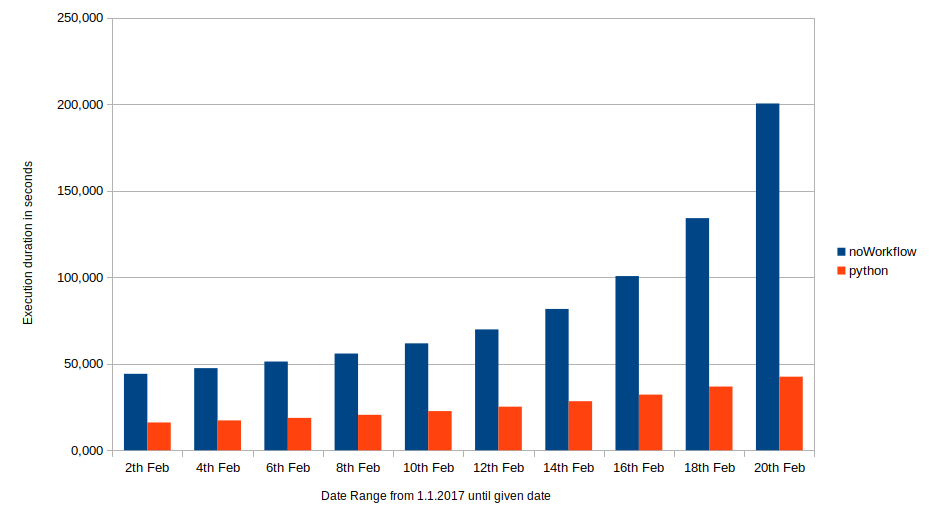
\includegraphics[width=\textwidth]{noworkflow_vs_python}
	\caption{Duration time of the job executions}
	\label{fig:noworkvspython} % \label has to be placed AFTER \caption (or \subcaption) to produce correct cross-references.
\end{figure}

Figure \ref{fig:noworkvspython} shows a diagram of the execution duration over the input date range. The python implementation has a smaller effect on the execution performance. The diagram shows that the gap between the execution duration gets bigger, if the amount of input data is bigger. Hence, the noWorkflow implementation is more inefficient on more bigger workloads. Table \ref{Tab:noworkflow} shows the average execution duration of both implementations. The average execution duration of noWorkflow, for the given jobs, is about 2 to 3 times bigger then from the python implementation.  

\begin{table}[]
	\caption{Average duration time of the job executions of the  noWorkflow and python implementation}
	\centering
	\begin{tabular}{l|l}
		\textbf{noWorkflow solution} & \textbf{python solution} \\ \hline
		84.779 s & 26.043 s \\ 
	\end{tabular}
	\label{Tab:noworkflow}
\end{table}

% summery ?

\chapter{Conclusion and future Work}\label{Conclusion}

\section{Conclusion}

In this thesis, the challenges of providing reproducibility in earth observation science have been explored. The solution consists of data identification and code identification for work-flows in the context of geosciences. The implementation within the OpenEO project proves the concept defined in Section \ref{Design}. It makes it clear that reproducibility can be achieved in earth observation work-flows by providing data identification and process identification. One reason why earth observation researchers lack on reproducibility is the additional time needed to achieve it. With the provided solution researchers can run experiments on EODC and automatically generate a data identifier that other scientists can use directly in their research. In addition the scientists can cite the version of the back end and describe the execution environment. On the other hand, reproducible processing is not a prior feature of the back end providers at the moment, therefore the solution had to be simple to apply to existing systems. The suggested solution consists of light-weight recommendations to the back end design. The provided meta-data in the presented prototype is capable for reproducing experiments theoretically, but are not supported by the EODC back end in an automated fashion. The design introduces a feature to compare different job executions to bring more transparency to the users. Applying the suggested additions is an advantage for back end providers, since they can provide execution information to scientists. Furthermore, the concept of easy to apply data citation and re-use may attract more users to use the back ends that provide the features of the concept. In the case of the OpenEO project, the development of it will lead to adoptions in the future. Therefore, the prototype of this thesis can be seen as a starting point of reproducibility in the OpenEO project rather than a final solution.  

\subsection{Research questions revisited}\label{research question revisited}

This section revisits the research questions defined in Section \ref{research question} to discuss how the concept design suit the questions.

\begin{itemize}
	\item \textbf{How can an earth observation job re-execution be applied like the initial execution?}
	\begin{itemize}
		\item \textbf{How can the used data be identified after the initial execution?} \\
		The input data is defined by the satellite data identifier and the filter operations used in the work-flow. This information with the hash of the resulting file list defines a unique query identified by a pid. The query data record consists of the original execution time-stamp to enable the retrieval of the same data versions. By assigning persistent identifiers to every unique used input data, the data can be accessed after the initial execution.    
		\item \textbf{How can the used software of the initial execution be reproduced?} \\
		The original software is defined by the used code, the programming language and the installed libraries. To identify the used code a version control system is needed. In the implementation Git and GitHub is used to identify and persist the used code version. The version of the programming language and the installed packages are stored in the job dependent context model. To reproduce the initial execution the back end has to recreate the captured versions of code and state of the programming language.       
		\item \textbf{What data has to be captured when?} \\
		The input data has to be captured at the query execution of the back end to ensure the equality of the persisted query and the original execution. The capturing of the code version has to be executed at the time of the execution, as well as the environment information of the execution. The hash of the resulting output file is calculated right after the creation of it.  
		\item \textbf{How can the result of a re-execution in future software versions be verified?} \\
		The solution persists a hash of the resulting output file. The result hash value of the re-execution is compared with the original execution output hash. If the hash values are not equal it can be assumed that the result of the re-execution is different from the initial execution. 
	\end{itemize}
	\item \textbf{How can the equality of an earth observation job re-execution results be validated?}
	\begin{itemize}
		\item \textbf{What are the validation requirements?} \\
		The validation requirements are the equality of the captured data. There are three parts that have to be considered by the validation. First the persistent input data identifier has to be the same between two executions. Second the code version. Third the hash value of the output file.
		\item \textbf{How can the data be compared?} \\
		The data is compared by the equality of all components of the context model. Every item of the context model is compared with the same item of the re-execution context model. There are only three states at the comparison defined: "EQUAL", "MISSING" or the difference of the context model element.
		\item \textbf{How can changes of the earth observation back end environment be recognized?} \\
		The timestamps of the back end provenance version is used to determine the version of the back end. Changes on job dependent environment results in different entries at the job dependent context model.  
		\item \textbf{How can differences in the environment between the executions be discovered?} \\
		The users can compare two job executions at the back end. The result is a JSON object that consists of all elements of the context model with the result of the comparison. In the resulting JSON it is evident, which part of the environment differs between the executions and how they are different.  
	\end{itemize}
\end{itemize}

\section{Future Work}\label{FutureWork}
This thesis proposed a prototype for applying reproducibility in the OpenEO project. Still there are major issues to be addressed in the development of the OpenEO project. 
OpenEO is still evolving until the official end of the project in 2021 and will be continued afterwards. There are a lot of features that have to be defined and may interfere with the concept proposed in this thesis. User defined functions (UDF) are part of the project, but not well defined yet. Reproducing executed UDFs may lead to adaptations of the concept. Another main issue of the OpenEO project is the billing concept that has to be apply-able to a diverse set of back ends. Since the capturing process and the generation of the context model needs resources, it has to be considered in the billing plan of the back ends. The growing diversity of the back ends applying the OpenEO standard is a huge challenge to remain the design of the context model suitable in the future. \\
The validation of the result with the hash of the result may lead to high duration times, so a better solution for validating the resulting file need to be developed.
In the solution of this work the meta-data is captured for identifying how jobs are executed and to be able to identify the provenance. A step further is a way to automatically apply the reproduction of an already executed job. A finer granularity of the process capturing is an possible addition to the concept, leading to a definition of scalability of the processing capturing. A concept to achieve this is presented in the Section \ref{Job:Benchmarking} below. 

\subsection{Benchmarking Mode}\label{Job:Benchmarking}

So far only the capturing of the whole process chain, including input and output data, are described. The general idea (presented in Section \ref{Implementation:Job dependent provenance}) of the job dependent provenance capturing is to capture the input data of the process graph, the whole process graph and the output of the process graph. This is a common concept the back end providers can agree on, since it is not affecting the back end providers implementations much. Moreover, it is capable of giving the user a simple overview of how the results are generated and what the differences between job executions are.To make the comparison of different execution behaviors more informative, the granularity of the capturing can be improved. \\
Therefore, the bench marking context model gets introduced. The idea is that not only the input data of the whole process chain and the output data gets captured, but every data state in between of each process. For every process in the process graph the input data, the output data and the code executing the process get captured. This makes it easier for users to see where in the process chain the execution actually produced different results.\\ The concept leads to higher implementation and execution costs at the back end side. The effect on the performance of the execution is higher than the common context model. Whether the implementation of such a granularity is  doable is highly dependent on the back end implementation. Not every back end might be able to implement this into the back end due to external tools where the execution and results of single processes are not distinguishable. If a back end can support it, the granularity can be finer. In an extreme example, the data and code can be captured for every line in the code. The flexibility of capturing granularity may define the context model design in the future.  

%\chapter{Appendix}\label{Appendix}

\backmatter

% Use an optional list of figures.
\listoffigures % Starred version, i.e., \listoffigures*, removes the toc entry.

% Use an optional list of tables.
\cleardoublepage % Start list of tables on the next empty right hand page.
\listoftables % Starred version, i.e., \listoftables*, removes the toc entry.

\lstlistoflistings

% Use an optional list of alogrithms.
%\listofalgorithms
%\addcontentsline{toc}{chapter}{List of Algorithms}

% Add an index.
\printindex

% Add a glossary.
\printglossaries

% Add a bibliography.
\bibliographystyle{abbrv}
\bibliography{intro}

\end{document}